
\chapter{Changes in 0.8}
\label{ch:08changes}

\section{Backwards compatibility with 0.7.3}
The 0.8 version is backwards compatible with 0.7.3 as tested on 
all the 80+ examples provided with the release.


\section{Assignment statements}
\label{sec:assignments}

So far assignments were performed together with declarations. 
The new \xelem{AssignStatement} element allows to loosen up this structure and 
do it more flexibly separately. 
For example the following snippet shows how to define a parameter, 
$k$, and subsequently how to assign an expression, $CL/V$, to it.
\begin{longtable}{cc}
\hline
\hline
option supported so far & new option in version 0.8 \\
\hline
\lstset{language=XML}
\begin{lstlisting}
    <!-- declaration & assignment -->
    <IndividualParameter symbId="k">
        <ct:Assign>
            <math:Binop op="divide">
                <ct:SymbRef symbIdRef="CL"/>
                <ct:SymbRef symbIdRef="V"/>
            </math:Binop>
        </ct:Assign>
    </IndividualParameter>
\end{lstlisting}
&
\lstset{language=XML}
\begin{lstlisting}
    <!-- declaration -->
    <IndividualParameter symbId="k"/>
    
    <!-- assignment, k=CL/V -->
    <ct:AssignStatement op="eq">
        <!-- LHS -->
        <ct:SymbRef symbIdRef="k"/>
        <!-- RHS -->
        <math:Binop op="divide">
            <ct:SymbRef symbIdRef="CL"/>
            <ct:SymbRef symbIdRef="V"/>
        </math:Binop>
    </ct:AssignStatement>
\end{lstlisting}
\\
\hline
\caption{Assignment statements are new in v0.8.}
\label{tab:comparisonAssignments}
\vspace{-1em}
\end{longtable}%
The assignment element is available in the covariate, parameter, structural 
and the observation models. It can be applied generally but will turn out to be 
especially useful in connection with the new conditional assignment 
statements, see section \ref{sec:conditionalStatements}.

\subsection{Assignment rules}
\begin{itemize}
\item 
One assignment per \xelem{AssignStatement} is allowed.
\item
Left and right hand sides of the assignment can be any expressions 
which evaluate to scalar values.
\item 
Parameters and variables used within the assignment statements
must the declared before, see for an example Table \ref{tab:comparisonAssignments} (right).
\item 
Only one assignment of each parameter or variable is allowed within a model, 
unless used in a conditional statement, see section \ref{subset:rulesCS}.
\end{itemize}


\section{Conditional statements}
\label{sec:conditionalStatements}

Conditional assignments are new in this version and provide additional
flexibility to the language. So far only piecewise statement were supported
which have the drawback that only single variables are assigned per statement.
Conditional assignments don't \marginpar{\HandCuffLeft} replace the existing 
piecewise statements, they are an entirely independent structure. 

Target tool vary in the support and scope of the conditional assignments, 
which is summarised below. 

\subsection{Tool coverage -- capabilities and restrictions}

\begin{itemize}
\item 
MLXTRAN, supports nested conditional \xatt{if-elseif-else-end} statements, e.g.
\lstset{language=MLX}
\begin{lstlisting}
	if (TIME  <=10 && ID == 1)
		G = a1
	elseif (TIME > 10 && ID == 1)
		G = a2
	elseif
		 ...
	end
\end{lstlisting}
%
%	T0=5
%	if t<T0
%		f=A
%	else
%		f= A*exp(-k*(t-T0))
%	end
with following features,  \cite{MLXTRANforMonolix:2014}, 
\begin{itemize}
\item 
Several \xatt{elseif} keywords can be chained, and the conditions are 
exclusive in sequence.
\item
A default value can be provided using the keyword \xatt{else}, but also 
as a simple definition preceding the conditional structure
\item
Only intermediate variables can be defined within conditional 
statements, the structure of the model cannot depend on such 
conditions.
\item
The derivatives of an ODE, or the PK elements of a prediction 
sub-model, cannot be defined within conditionals, e.g. the following 
is a valid MLXTRAN code
\lstset{language=MLX}
\begin{lstlisting}
	if t > T_end
		coeff = 0
	else
		coeff = 1
	end
	eta_cond = coeff*eta
	eps_cond = coeff*epsilon
	ddt_TC = s - d*TC - beta*(1-eta_cond)*TC*VL
	ddt_IC = beta*(1-eta_cond)*TC*VL - delta*IC
	ddt_VL = (1-eps_cond)*p*IC - c*VL
\end{lstlisting}
\end{itemize}
\item 
NMTRAN, \cite{NONMEM:2009}, allows nested conditional statements
with only few restrictions, the most important being
\begin{itemize}
\item 
NMTRAN doesn't accept nested conditional statements including 
random variables - described in 'NONMEM Users Guide - Part V', 
page 79, NONMEM 7.2. 
%This relevant discussion will be familiar to you
%\url{https://www.mail-archive.com/nmusers%40globomaxnm.com/msg04626.html}
\end{itemize}

\item 
winBUGS, \cite{Lunn:2009fk}
\begin{itemize}
\item 
supports only a step function of the form
\lstset{language=MLX}
\begin{lstlisting}
		step(e) 1 if e >= 0; 0 otherwise
\end{lstlisting}
where 'e' any expression
\item
Note however, that according to the winBUGS 
translation team in principle, thanks the Pascal language interface, almost 
any nested conditional statement can be implemented in WinBUGS. More
precisely single assignments are allowed only, see rule 2 in section \ref{subset:rulesCS}. 
\end{itemize}
\item
Common Converter, provided by Gareth Smith, Cyprotex is able to handle 
(nested) conditional statements. 
\end{itemize}

\subsection{Formulation}
The general form of the (nested) conditional statement looks as follows. 
\bigskip
\begin{algorithmic}
	\If {( condition1 )}
	    \State statement1
	\ElsIf{( condition2 )} 
	    \State statement2
	\ElsIf{( conditionN-1 )} 
	    \State statementN-1
	\Else
	    \State statementN
	\EndIf
\end{algorithmic}
\bigskip
The following definition of the conditional statement is based to large extend 
on the STAN specification, \cite{stan-manual:2015b}. \\
There must be a single leading \xatt{if} clause, which may be followed by any number of
\xatt{else if} clauses, all of which may be optionally followed by an \xatt{else} clause. Each
condition must be a TRUE or FALSE value. Nested \xatt{if-then-else} as part of each 
statement are allowed.

The entire sequence of \xatt{if-then-else} clauses forms a single conditional statement
for evaluation. The conditions are evaluated in order until one of the conditions
evaluates to a TRUE value, at which point its corresponding statement is executed
and the conditional statement finishes execution. If none of the conditions evaluates
to a TRUE value and there is a final \xatt{else} clause, its statement is executed.

\subsection{Rules for the use of conditional statements}
\label{subset:rulesCS}
There are few rules to follow when using conditional constructs in PharmML
coded models
\begin{enumerate}
\item
The conditionals are available in the covariate, parameter, structural 
and the observation models, similarly to the \emph{assignment statements}, described 
in section \ref{sec:assignments}.
\item
Allowed statement elements are 
\begin{itemize}
\item 
individual and population parameters
\item 
variables and random variables 
\item 
assignment statements
\item 
nested conditional statements
\end{itemize} 
\item
Parameters, variables assigned and/or referred to in a conditional 
statement must be declared outside the conditional in the first level of the according model block.
\item
Parameters or variables assigned within the conditional statement 
have to be referred to using the attribute \xatt{symbIdRef}. \\
In the following example the attribute \xatt{symbId} is used for the 
declaration of an population parameter
\lstset{language=XML}
\begin{lstlisting}
            <!-- 1. DECLARE 'k' using symbId-->
            <PopulationParameter symbId="k"/>
\end{lstlisting}
but a subsequent assignment requires the \xatt{symbIdRef} attribute 
(new in this version, not available for parameters or variables so far)
\lstset{language=XML}
\begin{lstlisting}
            <!-- 2. ASSIGN 'k' using symbIdRef -->
            <ConditionalStatement>
                <math:If>
                    <math:Condition>
                        <math:LogicBinop op="leq">
                            <ct:SymbRef symbIdRef="t"/>
                            <ct:Real>10</ct:Real>
                        </math:LogicBinop>
                    </math:Condition>
                    <PopulationParameter symbIdRef="k">
                        <ct:Assign>
                            <ct:Real>10</ct:Real>
                        </ct:Assign>
                    </PopulationParameter>
                </math:If>
                <math:Else>
                    <PopulationParameter symbIdRef="k">
                        <ct:Assign>
                            <ct:Real>5</ct:Real>
                        </ct:Assign>
                    </PopulationParameter>
                </math:Else>
            </ConditionalStatement>
\end{lstlisting}

\item
Parameters or variables assigned within the conditional statement 
cannot be assigned elsewhere unless such assignment is coupled 
with its declaration, e.g.
\lstset{language=XML}
\begin{lstlisting}
            <PopulationParameter symbId="k">
                <ct:Assign>
                    <ct:Real>10</ct:Real>
                </ct:Assign>
            </PopulationParameter>
\end{lstlisting}
The assignment of a parameter or variable within a conditional statement 
has precedence over the assignment coupled with its declaration. 
\item 
Neither PharmML nor libPharmML don't process the conditional statements
in any way -- the order of statements encoded in PharmML will be 
preserved when translating to a target tool.
\item 
libPharmML doesn't have the capability to evaluate conditional 
statements --  it is the responsibility of the user to define meaningful
and unambiguous way.
%setting variables/parameters to zero if not assigned.  For example
%\lstset{language=NM}
%\begin{lstlisting}
%IF (ROUTE.EQ.1) THEN 
%	FLGT = THETA(3) + ETA(2)
%	F1 = EXP(FLGT)/(1+EXP(FLGT))
%	KA = THETA(4)
%	ALAG1 = THETA(5)
%ELSE
%	F1 = 1		;others will be set to zero unless a value is specified here
%ENDIF
%\end{lstlisting}
\end{enumerate}
The use of the rules and principles is shown in the following example section. 

\subsection{Examples}
\label{subsec:examplesConditionals}


\subsubsection*{Example 1}
The first example underlines how important is to analyse the conditions and 
to make sure that they are mutually exclusive. Consider the following 
\bigskip
%RF=if (CLCR>0) then CLCR/6
%     elseif (AGE<=20) then 1
%     elseif (AGE>80) then 0.3
%     else -99
\begin{algorithmic}
	\If {$CLCR > 0$}
	    \State RF = CLCR/6
	\ElsIf{$ AGE \leq 20 $} 
	    \State RF = 1
	\ElsIf{$ AGE \geq 80 $} 
	    \State RF = 0.3
	\Else
	    \State RF = -99
	\EndIf
\end{algorithmic}
\bigskip
It follows from the above formulation, also visualised in Figure \ref{fig:CLCR_AGE},
that the condition domains are overlapping (are not mutually exclusive). 
The sequence of the first two conditions determines the value assigned 
to variable $RF$ (consider for example CLCR=3 and AGE=10).
\begin{figure}[ht!]
\centering
  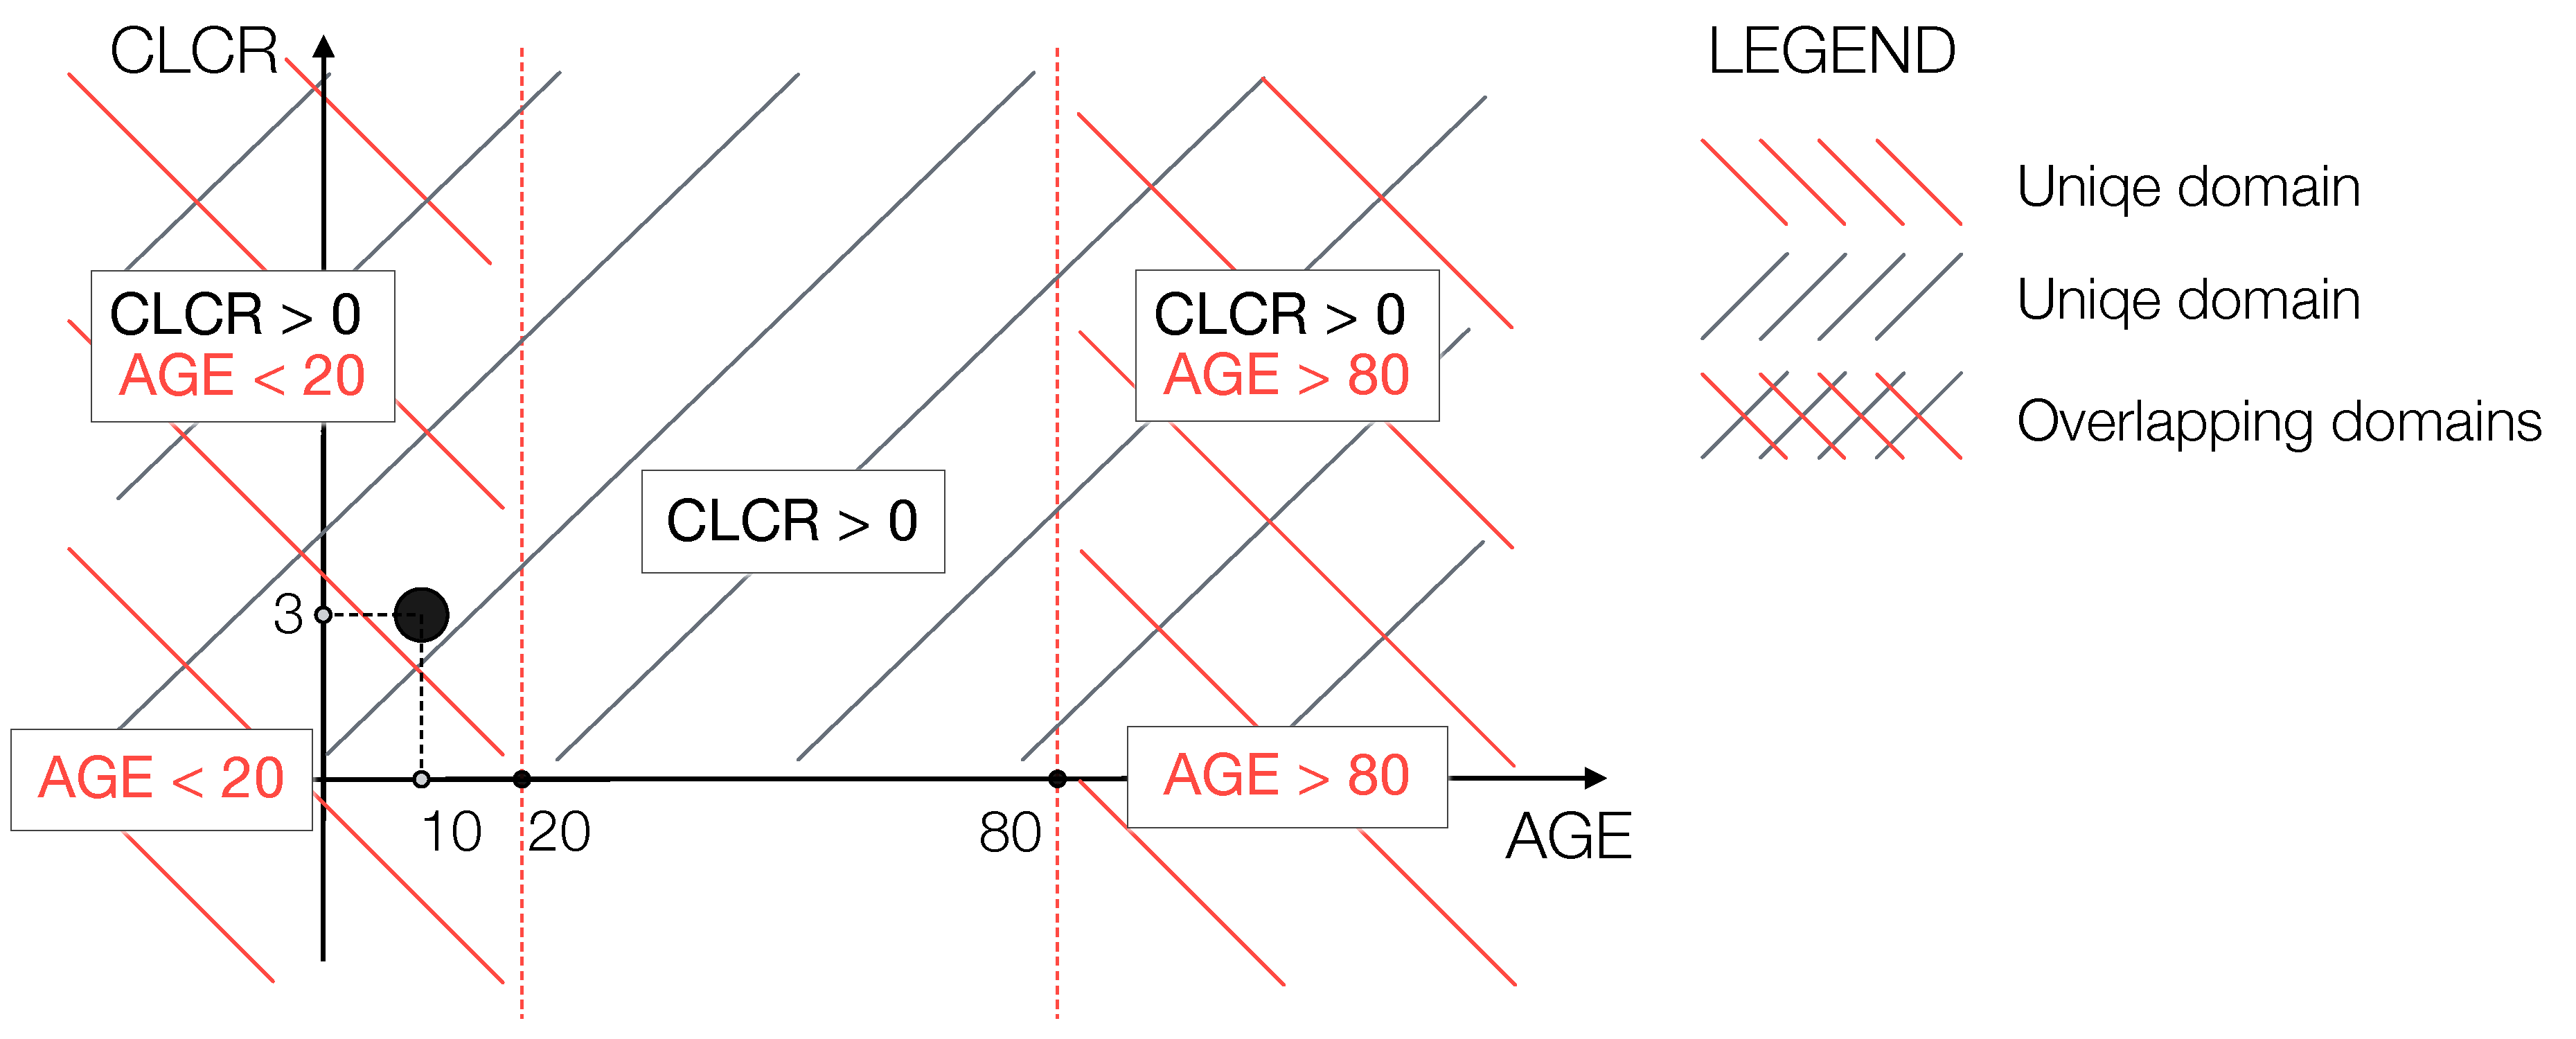
\includegraphics[width=90mm]{pics/CLCR_AGE.pdf}
 \caption{Domains for the conditions should be disjoint to avoid ambiguous
 assignments or the assignments have to be identical if domains overlap. 
 For example for CLCR=3 and AGE=10 the assignment of RF depends on the sequence 
 of the first two conditions.
 Because any domain declaration is allowed in PharmML, no automatic validity 
 check is performed,  the declarations are ultimately the responsibility of the modeller.}
 \label{fig:CLCR_AGE}
\end{figure}


\subsubsection*{Example 2}
The following conditional assignment 
%	{ ka = theta1 * exp(eta1)
%       ALAG1 = theta3} if Group == 1 
%     { ka = theta3 * exp(eta1)
%       ALAG1 = 0} if Group == 2
\begin{algorithmic}
	\If {$( Group = 1 )$}
	    \State $ka = \theta1 * \exp(\eta_1)$
	    \State $ALAG1 = \theta_3$
	\ElsIf {$( Group = 2 )$}
	    \State $ka = \theta_3 * \exp(\eta_1)$
	    \State $ALAG1 = 0$
	\EndIf
\end{algorithmic}
is assuming that $ka$ and $ALAG1$ are declared first, i.e.
\lstset{language=XML}
\begin{lstlisting}
            <!-- declaration -->
            <IndividualParameter symbId="ka"/>
            <IndividualParameter symbId="ALAG1"/>
\end{lstlisting}
and then the conditional assignments can be specified
\lstset{language=XML}
\begin{lstlisting}
            <!-- conditional assignments -->
            <ConditionalStatement>
                <math:If>
                    <math:Condition>
                        <math:LogicBinop op="eq">
                            <ct:SymbRef symbIdRef="Group"/>
                            <ct:Int>1</ct:Int>
                        </math:LogicBinop>
                    </math:Condition>
                    <ct:AssignStatement op="eq">
                        <ct:SymbRef symbIdRef="ka"/>
                        <math:Binop op="times">
                            <ct:SymbRef symbIdRef="theta1"/>
                            <math:Uniop op="exp">
                                <ct:SymbRef symbIdRef="eta1"/>
                            </math:Uniop>
                        </math:Binop>
                    </ct:AssignStatement>
                    <ct:AssignStatement op="eq">
                        <ct:SymbRef symbIdRef="ALAG1"/>
                        <ct:SymbRef symbIdRef="theta3"/>
                    </ct:AssignStatement>
                </math:If>
                <math:ElseIf>
                    <math:Condition>
                        <math:LogicBinop op="eq">
                            <ct:SymbRef symbIdRef="Group"/>
                            <ct:Int>2</ct:Int>
                        </math:LogicBinop>
                    </math:Condition>
                    <ct:AssignStatement op="eq">
                    <!-- omitted assignments for ka and ALAG1 -->
                </math:ElseIf>
            </ConditionalStatement>
\end{lstlisting}


\subsubsection*{Example 3}
This example, from Fisher/Shafer NONMEM course, \cite{fisher2007shafer}, 
shows parameter assignment conditional on a categorical covariate.

\lstset{language=NM}
\begin{lstlisting}
	IF (SEX.EQ.0) THEN
		V= THETA(1) * EXP(ETA(1)) ; volume in men
	ELSE
		V= THETA(2) * EXP(ETA(1)) ; volume in women
	ENDIF
\end{lstlisting}
Declare first the covariate, Sex
\lstset{language=XML}
\begin{lstlisting}
        <CovariateModel blkId="cm1">
            <Covariate symbId="Sex">
                <Categorical>
                    <Category catId="1">
                        <ct:Name>Female</ct:Name>
                    </Category>
                    <Category catId="0"/>
                </Categorical>
            </Covariate>
\end{lstlisting}
and condition on it the assignment of the individual parameter, V. Note that 
parameter V need to be declared first.
\lstset{language=XML}
\begin{lstlisting}
        <ParameterModel blkId="pm1">
            <IndividualParameter symbId="V"/>

            <PopulationParameter symbId="theta1"/>
            <PopulationParameter symbId="theta2"/>

            <RandomVariable symbId="eta1">
                <ct:VariabilityReference>
                    <ct:SymbRef symbIdRef="indiv"/>
                </ct:VariabilityReference>
                <!-- Distribution omitted -->
            </RandomVariable>
            <ConditionalStatement>
                <math:If>
                    <math:Condition>
                        <math:LogicBinop op="eq">
                            <ct:SymbRef symbIdRef="Sex"/>
                            <ct:CatRef catIdRef="0"/>
                        </math:LogicBinop>
                    </math:Condition>
                    <IndividualParameter symbIdRef="V">
                        <StructuredModel>
                            <PopulationValue>
                                <ct:Assign>
                                    <ct:SymbRef symbIdRef="theta1"/>
                                </ct:Assign>
                            </PopulationValue>
                            <RandomEffects>
                                <ct:SymbRef symbIdRef="eta1"/>
                            </RandomEffects>
                        </StructuredModel>
                    </IndividualParameter>
                </math:If>
                <math:Else>
                    <IndividualParameter symbIdRef="V">
                        <StructuredModel>
                            <PopulationValue>
                                <ct:Assign>
                                    <ct:SymbRef symbIdRef="theta2"/>
                                </ct:Assign>
                            </PopulationValue>
                            <RandomEffects>
                                <ct:SymbRef symbIdRef="eta1"/>
                            </RandomEffects>
                        </StructuredModel>
                    </IndividualParameter>
                </math:Else>
            </ConditionalStatement>
            ...
        </ParameterModel>
\end{lstlisting}


%\subsubsection*{Example 4}
%
%Source: Fisher/Shafer NONMEM course, \cite{fisher2007shafer}.
%
%\lstset{language=NM}
%\begin{lstlisting}
%	IF(CP.GE.PCP) THEN
%		SLOPE = (CP-PCP)/DT1
%		DELTA=DT1*SLOPE+(KE0*PCP-SLOPE)*(1-EXP(-KE0*DT1))/KE0
%	ELSE
%		SLOPE = (LOG(CP)-LOG(PCP))/DT1
%		DELTA=PCP*KE0/(KE0+SLOPE)*(EXP(DT1*SLOPE)-EXP(-KE0*DT1))
%	ENDIF
%\end{lstlisting}
%
%\lstset{language=XML}
%\begin{lstlisting}
%
%\end{lstlisting}
%
%\lstset{language=NM}
%\begin{lstlisting}
%IF (ROUTE.EQ.1) THEN ;extravascular parameters
%	FLGT = THETA(3) + ETA(2) ;only use additive error here to allow negative values
%	F1 = EXP(FLGT)/(1+EXP(FLGT)) ;logit transform to keep F between 0 and 1
%	KA = THETA(4)
%	ALAG1 = THETA(5)
%ELSE
%	F1 = 1
%	;others will be set to zero unless a value is specified here
%ENDIF
%\end{lstlisting}


\subsubsection*{Example 4 -- Three Compartment Infusion, Coefficient and Exponents }

Source: Fisher/Shafer NONMEM course, \cite{fisher2007shafer}. The NMTRAN code for the 
structural and observation model reads
\lstset{language=NM}
\begin{lstlisting}
	; C1, C2, C3, L1, L2, L3, RATE, DUR defined elsewhere
	IF (TIME.LE.DUR) THEN
		TY1 = RATE*C1/L1*(1-EXP(-L1*TIME))
		TY2 = RATE*C2/L2*(1-EXP(-L2*TIME))
		TY3 = RATE*C3/L3*(1-EXP(-L3*TIME))
	ELSE
		TY1 = RATE*C1/L1*(1-EXP(-L1*DUR))*EXP(-L1*(TIME-DUR))
		TY2 = RATE*C2/L2*(1-EXP(-L2*DUR))*EXP(-L2*(TIME-DUR))
		TY3 = RATE*C3/L3*(1-EXP(-L3*DUR))*EXP(-L3*(TIME-DUR))
	ENDIF

	Y=(TY1+TY2+TY3)*(1+EPS(1)) ; Constant CV model
\end{lstlisting}
\bigskip
and in PharmML 
\lstset{language=XML}
\begin{lstlisting}
    <!-- STRUCTURAL MODEL -->
    <StructuralModel blkId="sm1">
        
        <ct:Variable symbolType="real" symbId="TY1"/>
        <ct:Variable symbolType="real" symbId="TY2"/>
        <ct:Variable symbolType="real" symbId="TY3"/>
        
        <ConditionalStatement>
            <math:If>
                <math:Condition>
                    <math:LogicBinop op="leq">
                        <ct:SymbRef symbIdRef="t"/>
                        <ct:SymbRef symbIdRef="DUR"/>
                    </math:LogicBinop>
                </math:Condition>
                <!-- TY1 = RATE*C1/L1*(1 - EXP(-L1*TIME)) -->
                <ct:AssignStatement op="eq">
                    <ct:SymbRef symbIdRef="TY1"/>
                    <!-- omitted RHS expression -->
                </ct:AssignStatement>
                <!-- TY2 = RATE*C2/L2*(1-EXP(-L2*TIME)) -->
                <ct:AssignStatement op="eq">
                    <ct:SymbRef symbIdRef="TY2"/>
                    <!-- omitted RHS expression -->
                </ct:AssignStatement>
                <ct:AssignStatement op="eq">
                    <ct:SymbRef symbIdRef="TY3"/>
                    <!-- omitted RHS expression -->
                </ct:AssignStatement>
            </math:If>
            <math:Else>
                <!-- TY1 = RATE*C1/L1*(1-EXP(-L1*DUR))*EXP(-L1*(TIME-DUR)) -->
                <ct:AssignStatement op="eq">
                    <ct:SymbRef symbIdRef="TY1"/>
                    <!-- omitted RHS expression -->
                </ct:AssignStatement>
                <!-- TY2 = RATE*C2/L2*(1-EXP(-L2*DUR))*EXP(-L2*(TIME-DUR)) -->
                <ct:AssignStatement op="eq">
                    <ct:SymbRef symbIdRef="TY2"/>
                    <!-- omitted RHS expression -->
                </ct:AssignStatement>
                <!-- TY3 = RATE*C3/L3*(1-EXP(-L3*DUR))*EXP(-L3*(TIME-DUR)) -->
                <ct:AssignStatement op="eq">
                    <ct:SymbRef symbIdRef="TY3"/>
                    <!-- omitted RHS expression -->
                </ct:AssignStatement>
                
            </math:Else>
        </ConditionalStatement>
\end{lstlisting}
\bigskip
The observation model is skipped here.


%\subsubsection*{Example 6 -- sleep model}
%
%\begin{itemize}
%\item
%Type of observed variable -- discrete / ordered categorical
%\item
%Category variable: $Y$
%\item
%Set of categories: $\{0,1,2,3,4,5\}$
%\item
%Probabilities
%\begin{align}
%& P(Y=1) = \exp(G1)/(1+\exp(G1)+\exp(G2)+\exp(G3)) \nonumber \\
%& P(Y=2) = \exp(G2)/(1+\exp(G1)+\exp(G2)+\exp(G3)) \nonumber \\
%& P(Y=3) = 0 \nonumber \\
%& P(Y=4) = 0 \nonumber \\
%& P(Y=5) = \exp(G3)/(1+\exp(G1)+\exp(G2)+\exp(G3)) \nonumber
%\end{align}
%\end{itemize}
%
%
%\lstset{language=NM}
%\begin{lstlisting}
%; Sleep model with multinomial logistic functions
%; Transitions from awake state
%; Categorical data model - 4 categories
%
%removed multiple assignments and definitions
%
%IF (STT.LE.BPsb.AND.SL.EQ.1) THEN
%    G1A=(TVG1A+ETA(1))*(BPsb-STT)/(BPsb-BPsa)+(TVG1A+ETA(1)+STE1b)*(STT-BPsa)/(BPsb-BPsa)
%	...
%    G1B=(TVG1B+ETA(1))*(BPsb-STT)/(BPsb-BPsa)+(TVG1B+ETA(1)+STE1b)*(STT-BPsa)/(BPsb-BPsa)
%	...
%    G1C=(TVG1C+ETA(1))*(BPsb-STT)/(BPsb-BPsa)+(TVG1C+ETA(1)+STE1b)*(STT-BPsa)/(BPsb-BPsa)
%	...
%ENDIF
%
%IF (STT.GT.BPsb.AND.SL.EQ.1) THEN
%    G1A=(TVG1A+ETA(1)+STE1b)*(BPsc-STT)/(BPsc-BPsb)+(TVG1A+ETA(1)+STE1c)*(STT-BPsb)/(BPsc-BPsb)
%    ...
%
%    G1B=(TVG1B+ETA(1)+STE1b)*(BPsc-STT)/(BPsc-BPsb)+(TVG1B+ETA(1)+STE1c)*(STT-BPsb)/(BPsc-BPsb)
%    ...
%
%    G1C=(TVG1C+ETA(1)+STE1b)*(BPsc-STT)/(BPsc-BPsb)+(TVG1C+ETA(1)+STE1c)*(STT-BPsb)/(BPsc-BPsb)
%    ...
%ENDIF
%
%
%IF (TIME.GE.BPA.AND.TIME.LE.BPB.AND.SL.EQ.1) THEN
%    G1=G1A*(BPB-TIME)/(BPB-BPA)+G1B*(TIME-BPA)/(BPB-BPA)
%    ...
%ENDIF
%
%IF (TIME.GT.BPB.AND.TIME.LE.BPC.AND.SL.EQ.1) THEN
%    G1=G1B*(BPC-TIME)/(BPC-BPB)+G1C*(TIME-BPB)/(BPC-BPB)
%    ...
%ENDIF
%
%
%  IF (TIME.GE.BP1.AND.TIME.LE.BP2.AND.SL.EQ.0) THEN - sleep part of the night; from 1 < x < 2
%    G1=(TVG11+ETA(4))*(BP2-TIME)/(BP2-BP1)+(TVG12+ETA(4))*(TIME-BP1)/(BP2-BP1)
%    ...
%  ENDIF
%
%  IF (TIME.GT.BP2.AND.TIME.LE.BP3.AND.SL.EQ.0) THEN - sleep part of the night; from 2 < x < 3
%    G1=(TVG12+ETA(4))*(BP3-TIME)/(BP3-BP2)+(TVG13+ETA(4))*(TIME-BP2)/(BP3-BP2)
%    ...
%  ENDIF
%\end{lstlisting}
%
%
%%%%%%%%%%%%%%%%%%%%%%%%%%%%%%%%%%%%%%%%%%%%%%%%%%%%%%%
\section{Nested piecewise}
\label{sec:nestedPiecewise}
Nesting of piecewise statements was not supported so far, here a typical one

\bigskip
$f(x) = \left\{ 
\begin{array}{ccl}
\left\{ 
\begin{array}{rcl}
1 & \mbox{for} & x<1 \\ 
2 & \mbox{else} 
\end{array}\right. & \mbox{for} & x>0 \\ 
3 & \mbox{else} 
\end{array}\right.$
\bigskip \\
implemented in PharmML as the following snippet shows
\lstset{language=XML}
\begin{lstlisting}
        <ct:Variable symbolType="real" symbId="f">
            <ct:Assign>
                <ct:Piecewise>
                    <math:Piece>
                        <!-- nested piecewise -->
                        <math:Piecewise>
                            <math:Piece>
                                <ct:Real>1</ct:Real>
                                <math:Condition>
                                    <math:LogicBinop op="lt">
                                        <ct:SymbRef symbIdRef="x"/>
                                        <ct:Real>1</ct:Real>
                                    </math:LogicBinop>
                                </math:Condition>
                            </math:Piece>
                            <math:Piece>
                                <ct:Real>2</ct:Real>
                                <math:Condition>
                                    <math:Otherwise/>
                                </math:Condition>
                            </math:Piece>
                        </math:Piecewise>
                        <math:Condition>
                            <math:LogicBinop op="gt">
                                <ct:SymbRef symbIdRef="x"/>
                                <ct:Real>0</ct:Real>
                            </math:LogicBinop>
                        </math:Condition>
                    </math:Piece>
                    <math:Piece>
                        <ct:Real>3</ct:Real>
                        <math:Condition>
                            <math:Otherwise/>
                        </math:Condition>
                    </math:Piece>
                </ct:Piecewise>
            </ct:Assign>
        </ct:Variable>
\end{lstlisting}


%%%%%%%%%%%%%%%%%%%%%%%%%%%%%%%%%%%%%%%%%%%%%%%%%%%%%%%
\section{Probability functions support}
\label{sec:probabFunctions}
Following probability functions are available 
\begin{itemize}
\item 
CDF(x) -- cumulative distribution function, \xelem{CDF}
\item 
PDF(x) -- probability density function, \xelem{PDF}
\item 
HF(x) -- hazard function, \xelem{HF}
\item 
SF(x) -- survival function, \xelem{SF}
\end{itemize}
\bigskip
The implementation of these probability functions is straightforward, despite
their often very complex expressions which are only referred to, and 
requires the use of the 
\begin{enumerate}
\item 
according XML element, e.g. \xelem{CDF}
\item 
specification of the distribution of interest and
\item 
function argument, x, which can be any expression.
\end{enumerate}
The introduction of these generic elements allow to use any of the 
ProbOnto univariate continuos distributions, \cite{ProbOnto:2015a}.
Consider for example the cumulative distribution
function, \emph{PHI}, of the standard normal distribution with mean 0
and standard deviation 1 which the two basic function read
\begin{align*}
\mbox{PDF}:  \quad f(x) &= \frac{e^{-\frac{1}{2} x^2}}{\sqrt{2\pi}} \nonumber \\
\mbox{CDF}:  \quad F(x) &= \frac12\left[1 + \text{erf}\left( \frac{x}{\sqrt{2}}\right)\right] \nonumber
\end{align*}
with \emph{erf}\footnote{Error function, $erf$, \url{mathworld.wolfram.com/Erf.html}}
defined as
\begin{equation*}
\text{erf}(z) = \frac{2}{\pi}\int_0^z e^{-t^2} dt
\end{equation*}

\bigskip
The abbreviated XML code explains its encoding which reduces to the 
specification of the distribution name, \emph{StandardNormal1} and the 
argument
\lstset{language=XML}
\begin{lstlisting}
    <ct:Variable symbolType="real" symbId="PHI">
        <ct:Assign>
            <math:CDF>
                <math:Distribution>
                    <po:ProbOnto name="StandardNormal1"/>
                </math:Distribution>
                <ct:Assign>
                <!-- x, argument -->
                </ct:Assign>
            </math:CDF>
        </ct:Assign>
    </ct:Variable>
\end{lstlisting}
Note, that CDF of the standard normal is straightforward as it doesn't
requiere specification of parameters, which are by default 
$mean\!=\!0$ and $stdev\!=\!1$. 
The use of probability functions is explained in the following example 
in the context of a model proposed for handling data below the level 
of quantification, BLQ, \cite{Beal:2001}.


\subsection{Example 1 -- basic example}
Source: Part VII, Help Guide of the \cite{NONMEM:2009}.
The cumulative distribution function, \emph{PHI}, of the standard normal 
distribution with mean 0 and standard deviation 1, may be used as in 
this is basic example
\lstset{language=NM}
\begin{lstlisting}
	A=THETA(1)*EXP(ETA(1))
	B=PHI(A)
\end{lstlisting}

\begin{longtable}{cc}
\hline
$A = \theta_1 \exp(\eta_1)$
&
\lstset{language=XML}
\begin{lstlisting}
<IndividualParameter symbId="A">
    <ct:Assign>
        <math:Binop op="times">
            <ct:SymbRef symbIdRef="THETA1"/>
            <math:Uniop op="exp">
                <ct:SymbRef symbIdRef="ETA1"/>
            </math:Uniop>
        </math:Binop>
    </ct:Assign>
</IndividualParameter>
\end{lstlisting}
\\
 \hline
$B = \mbox{CDF}(A)$
 &
 \lstset{language=XML}
\begin{lstlisting}
        <IndividualParameter symbId="B">
            <ct:Assign>
                <math:CDF>
                    <math:Distribution>
                        <po:ProbOnto name="StandardNormal1"/>
                    </math:Distribution>
                    <ct:Assign>
                        <ct:SymbRef symbIdRef="A"/>
                    </ct:Assign>
                </math:CDF>
            </ct:Assign>
        </IndividualParameter>
\end{lstlisting}
\\
\hline
\caption{Encoding of the basic example using cumulative distribution function, CDF.}
\end{longtable}%


\subsection{Example 2 -- M3-method for handling of BLQ data}
According to \cite{Beal:2001}, the likelihood for a censored observation 
at time t, is given by 
\begin{align*}
l(t) = \Phi((QL - f(t))/\sqrt{g(t)}), \quad \mbox{with } \Phi \mbox{ the CDF of the } \mathcal{N}(0,1)
\end{align*}
which is the probability that the observation is BQL, (i.e., is between 
$-\infty$ and quantification limit, QL.\\
An example how to implement the so-called M3-method for handling 
of such data
provides the tutorial by \cite{Mould_partII:2013} with the following 
NMTRAN from the supplementary material of the paper.
\lstset{language=NM}
\begin{lstlisting}
	$ERROR ; Beal Method 3
	;residual error is coded here using THETA's rather than EPS's
	ADD = THETA(6)
	PROP = F*THETA(7)
	SD = SQRT(ADD*ADD+PROP*PROP) ; combined error model
	LLOQ=0.05 ; lower limit of quantification
	IF (BLQ.EQ.0) THEN
		F_FLAG=0 ;regular likelihood for measured concentrations
		Y = F + SD*EPS(1)
	ENDIF
	IF (BLQ.EQ.1) THEN
		F_FLAG=1 ;probability that F is less than LLOQ for missing concentrations
		Y=PHI((LLOQ-F)/SD)
	ENDIF
\end{lstlisting}
While the first couple of lines are standard and will be omitted
here, the encoding of the essential line with PHI function, 
Y=PHI((LLOQ-F)/SD), is shown in the following snippet
\lstset{language=XML}
\begin{lstlisting}
        <ObservationModel blkId="om4">
            <ContinuousData>
	        <!-- Y=PHI((LLOQ-F)/SD) -->
                <General symbId="Y">
                    <ct:Assign>
                        <math:CDF>
                            <math:Distribution>
                                <po:ProbOnto name="StandardNormal1"/>
                            </math:Distribution>
                            <ct:Assign>
                                <math:Binop op="divide">
                                    <math:Binop op="minus">
                                        <ct:SymbRef symbIdRef="LLOQ"/>
                                        <ct:SymbRef blkIdRef="sm1" symbIdRef="F"/>
                                    </math:Binop>
                                    <ct:SymbRef symbIdRef="SD"/>
                                </math:Binop>
                            </ct:Assign>
                        </math:CDF>
                    </ct:Assign>
                </General>
            </ContinuousData>
        </ObservationModel>
\end{lstlisting}
As before, the encoding of the CDF of the standard normal doesn't
require the specification of default, $mean\!=\!0$ and $stdev\!=\!1$, parameters. 

\subsection{Example 3 -- TTE model}
\label{subsec:TTEmodel}
The probability functions turn out to be very useful in encoding 
of time-to-event data. While so far encoding of hazard or survival functions
formulas was the only option, they offer a quick and safe way to encode often complex 
function of interest as the following example demonstrates 
\lstset{language=XML}
\begin{lstlisting}
            <HazardFunction symbId="h2">
                <ct:Assign>
                    <math:HF>
                        <math:Distribution>
                            <ProbOnto xmlns="http://www.pharmml.org/probonto/ProbOnto" name="Weibull1">
                                <Parameter name="scale">
                                    <ct:Assign>
                                        <ct:SymbRef blkIdRef="pm1" symbIdRef="beta"/>
                                    </ct:Assign>
                                </Parameter>
                                <Parameter name="shape">
                                    <ct:Assign>
                                        <ct:SymbRef blkIdRef="pm1" symbIdRef="lambda"/>
                                    </ct:Assign>
                                </Parameter>
                            </ProbOnto>
                        </math:Distribution>
                        <ct:Assign>
                            <ct:SymbRef symbIdRef="t"/>
                        </ct:Assign>
                    </math:HF>
                </ct:Assign>   
            </HazardFunction>
\end{lstlisting}

%\begin{figure}[ht!]
%\centering
%%  \includegraphics[width=140mm]{pics/...}
%	MISSING PICTURE HERE
% \caption{Mapping of BLQ data and observation models.}
% \label{fig:BLQmapping}
%\end{figure}

%
%\newpage
%%%%%%%%%%%%%%%%%%%%%%%%%%%%%%%%%%%%%%%%%%%%%%%%%%%%%%%
\section{Samples -- nonparametric distributions support}
\label{sec:nonParamDistribs}

%ADD FIGURE \\
%ADD FIGURE \\
%ADD FIGURE \\
%ADD FIGURE \\
%and explanation about sample encoding, place where its encoded and its mapping

When formulating models it is often not possible to specify a probability 
distribution using a parametric distribution because its defining
functions are not known. Instead, a set of values can be considered 
as constituting a distribution model.

\emph{Samples} are sets of realisations obtained from a known or unknown 
distribution and following UncertML \cite{uncertml3:2014} we distinguish between 
\begin{itemize}
\item 
Random sample, \xelem{RandomSample}
\item 
Systematic sample, \xelem{SystematicSample}
\item 
Unknown sample, \xelem{UnknownSample}
\end{itemize}
The only (optional) parameter which can be used is  
\begin{itemize}
\item 
\xatt{weight} -- to encode weighting given to each realisation.
\end{itemize}
The main type which should be used for our purposes is the first one defined as
\begin{description}
\item[Random Sample] -- a set of independent realisations, $x_i$, drawn from 
a probability distribution $p(x)$ (or alternatively a population where every 
member has an equal chance of being drawn, but is randomly selected). 
The sample will typically be obtained using some form of simulation algorithm 
for distributions using a random number generator. 
\end{description}
See also ProbOnto specification for more details, \cite{ProbOnto:2015a}.

%%%%%%%%%%%%%%%%%%%%%%%%%%%%%%%%%%%%%%%%%%%%%%%%%%%%%%%
\subsection{Two modes of operation}
There are two ways samples can be encoded in PharmML, Table \ref{tab:twoOptionsForSamples}:
\begin{itemize}
\item 
Option 1: Data stored together with the corresponding parameter
\item 
Option 2: Data stored in \xelem{TrialDesign}
\end{itemize}
Both encoding result in exact the same model. In both cases the mapping 
between data column and parameters is essential to make sure proper 
definition. 
\newpage
\begin{longtable}{c}
\hline
\hline
Option 1: Data stored together with parameter \\
\hline
\lstset{language=XML}
\begin{lstlisting}
    <ParameterModel blkId="PM1">
        <PopulationParameter symbId="POP_K">
            <Distribution>
                <po:ProbOnto name="RandomSample">
                    <po:ColumnMapping>
                        <ds:ColumnRef columnIdRef="POP_K_sample"/>
                        <ct:SymbRef symbIdRef="POP_K"/>
                    </po:ColumnMapping>
                    <ds:DataSet>
                        <ds:Definition>
                            <ds:Column columnId="POP_K_sample" valueType="real" columnNum="1"/>
                        </ds:Definition>
                        <ds:Table>
                            <ds:Row><ct:Real>0.10</ct:Real></ds:Row>
                            <!-- values omitted -->
                        </ds:Table>
                    </ds:DataSet>
                </po:ProbOnto>
            </Distribution>
        </PopulationParameter>

        <!-- ALTERNATIVE - short version -->
        <PopulationParameter symbId="POP_K">
            <Distribution>
                <po:ProbOnto name="RandomSample">
                    <ds:DataSet>
                        <ds:Table>
                            <ds:Row><ct:Real>0.10</ct:Real></ds:Row>
                            <!-- values omitted -->
                        </ds:Table>
                    </ds:DataSet>
                </po:ProbOnto>
            </Distribution>
        </PopulationParameter>
    </ParameterModel>
\end{lstlisting}
\\
\hline
Option 2: Data stored in \xelem{TrialDesign} 
\\
\hline
\lstset{language=XML}
\begin{lstlisting}
<!-- PART 1 -->
<ParameterModel blkId="PM2">
    <PopulationParameter symbId="POP_K">
        <Distribution>
            <po:ProbOnto name="RandomSample"/>                    
        </Distribution>
    </PopulationParameter>            
</ParameterModel>

<!-- PART 2 -->
<TrialDesign xmlns="http://www.pharmml.org/pharmml/0.7/TrialDesign">    
    <ExternalDataSet oid="RdataSet">
        <ColumnMapping>
            <ds:ColumnRef columnIdRef="POP_K_sample"/>
            <ct:SymbRef blkIdRef="PM2" symbIdRef="POP_K"/>
        </ColumnMapping>
        <ds:DataSet>
            <ds:Definition>
                <ds:Column columnId="POP_K_sample" valueType="real" columnNum="1"/>
            </ds:Definition>
            <ds:Table>
                <ds:Row><ct:Real>0.10</ct:Real></ds:Row>
                <!-- values omitted -->
            </ds:Table>
        </ds:DataSet>
    </ExternalDataSet>
</TrialDesign>
\end{lstlisting}
\\
\hline
\caption{Two way to encode samples. 
Option 1: data stored together with parameter declaration in \xelem{ModelDefinition}.
Two version are shown: (top) with full data/model mapping and dataset column 
declaration, (bottom) short form when only one dataset is required - mapping and 
column declaration are redundant. Option 2: data stored in the \xelem{TrialDesign}.}
\label{tab:twoOptionsForSamples}
\end{longtable}%

%\begin{longtable}{cc}
%\hline
%\hline
%  \multicolumn{2}{c}{Option 2: Data stored in \xelem{TrialDesign}} 
%\\
%\hline
%\lstset{language=XML}
%\begin{lstlisting}
%<!-- PART 1 -->
%<ParameterModel blkId="PM2">
%    <PopulationParameter symbId="POP_K">
%        <Distribution>
%            <po:ProbOnto name="RandomSample"/>                    
%        </Distribution>
%    </PopulationParameter>            
%</ParameterModel>
%
%<!-- PART 2 -->
%<TrialDesign xmlns="http://www.pharmml.org/pharmml/0.7/TrialDesign">    
%    <ExternalDataSet oid="RdataSet">
%        <ColumnMapping>
%            <ds:ColumnRef columnIdRef="POP_K_sample"/>
%            <ct:SymbRef blkIdRef="PM2" symbIdRef="POP_K"/>
%        </ColumnMapping>
%        <ds:DataSet>
%            <ds:Definition>
%                <ds:Column columnId="POP_K_sample" valueType="real" columnNum="1"/>
%            </ds:Definition>
%            <ds:Table>
%                <ds:Row><ct:Real>0.10</ct:Real></ds:Row>
%                <ds:Row><ct:Real>0.23</ct:Real></ds:Row>
%                <ds:Row><ct:Real>0.3</ct:Real></ds:Row>
%            </ds:Table>
%        </ds:DataSet>
%    </ExternalDataSet>
%</TrialDesign>
%\end{lstlisting}
%\\
%\hline
%\caption{Option 2: data stored in the \xelem{TrialDesign}.}
%\label{tab:twoOptionsForSamples}
%\end{longtable}%


%%%%%%%%%%%%%%%%%%%%%%%%%%%%%%%%%%%%%%%%%%%%%%%%%%%%%%%
\subsection{Mapping without \xatt{weight} parameter}

%%%%%%%%%%%%%%%%%%%%%%%%%%%%%%%%%%%%%%%%%%%%%%%%%%%%%%%
\subsubsection*{Option 1}
\label{subsec:exp2}
Sometimes the \xatt{weight} parameter is not defined and the assumption 
is that all values are equally probable with $p=1/n$ where
$n$ equal the row numbers, see Table \ref{tab:randomSample_withoutWeight}.

\begin{longtable}{c}
\hline
\hline
POP\_V \\
\hline
5.050013 \\
5.064166 \\
5.078318 \\ 
... \\
\hline
\caption{Test data set represented using equiprobable samples. Because no \xatt{weight} parameter
is defined, the assumption is that all values are equally probable with $p=1/n$ where
$n$ is equal the row numbers.}
\label{tab:randomSample_withoutWeight}
\end{longtable}%

\lstset{language=XML}
\begin{lstlisting}
    <PopulationParameter symbId="POP_K">
        <Distribution>
            <po:ProbOnto name="RandomSample">
                <ds:DataSet>
                    <ds:Table>
                        <ds:Row><ct:Real>0.10</ct:Real></ds:Row>
                        <ds:Row><ct:Real>0.23</ct:Real></ds:Row>
                        <ds:Row><ct:Real>0.3</ct:Real></ds:Row>
                    </ds:Table>
                    <!-- <ds:ExternalFile oid="sxtData">
                        <ds:path>POP_K_sample.csv</ds:path>
                    </ds:ExternalFile>-->
                </ds:DataSet>
            </po:ProbOnto>
        </Distribution>
    </PopulationParameter>
\end{lstlisting}
Here the short version was used which is applicable when only one data 
column in required. Providing mapping and column definition is in such
cases redundant, unless the data is stored in \xelem{TrialDesign}, see below.

\subsubsection*{Option 2}
\label{subsec:exp1}
%Sometimes the \xatt{weight} parameter is not defined and the assumption 
%is that all values are equally probable with $p=1/n$ where
%$n$ equal the row numbers, see Table \ref{tab:randomSampleExternalwithoutWeight}
%and Figure \ref{fig:Mapping_singleParam_noWeights}.
Figure \ref{fig:Mapping_singleParam_noWeights} shows how to store and
map dataset  with samples declared in \xelem{TrialDesign} to a parameter 
defined in \xelem{ParameterModel}, here $POP\_V$. In this case column mapping and 
column declaration are required.


\begin{figure}[ht!]
\centering
  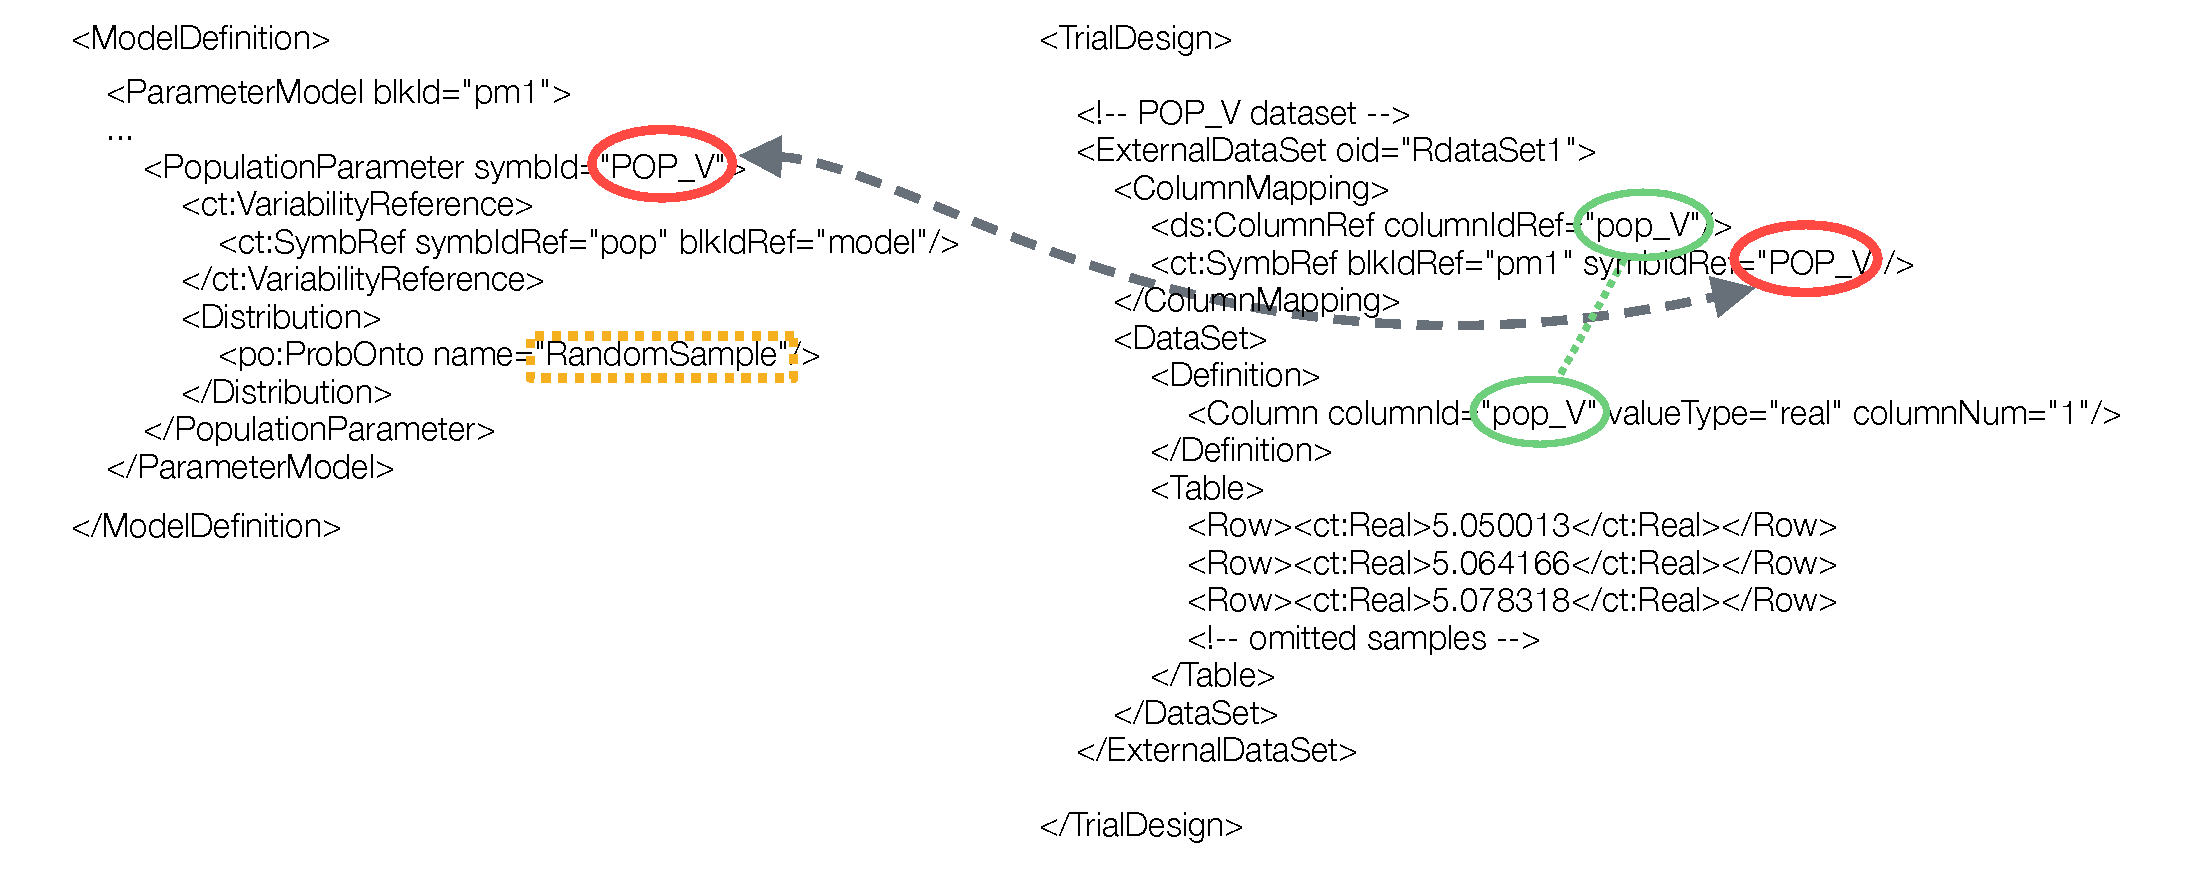
\includegraphics[width=140mm]{pics/Mapping_singleParam_noWeights}
 \caption{Mapping of samples without weights -- explained graphically.}
 \label{fig:Mapping_singleParam_noWeights}
\end{figure}


%%%%%%%%%%%%%%%%%%%%%%%%%%%%%%%%%%%%%%%%%%%%%%%%%%%%%%%
\subsection{Mapping with \xatt{weight} parameter}
\label{subsec:exp5}

\subsubsection*{Option 1}
\label{subsec:exp2}

In the case when single variables are defined with \xatt{weight} parameter, $p$.
\begin{longtable}{cc}
\hline
\hline
P	& POP\_K \\
\hline
0.25	& 0.10 \\
0.25	& 0.23 \\
0.5	& 0.3 \\ 
\hline
\caption{This data set represents sample use case with \xatt{weight} parameter, $P$.}
\label{tab:randomSampleInline}
\end{longtable}%
Here the according samples are encoded directly with the parameter of interest. 
The mapping is self-explanatory. The samples can be encoded either inline, using 
\xelem{Table}, or in external datasets referenced within the \xelem{ExternalFile} element.
\lstset{language=XML}
\begin{lstlisting}
    <PopulationParameter symbId="p"/>
    <PopulationParameter symbId="POP_K">
        <Distribution>
            <po:ProbOnto name="RandomSample">
                <po:Parameter name="weight">
                    <ct:Assign>
                        <ct:SymbRef symbIdRef="p"/>
                    </ct:Assign>
                </po:Parameter>
                <po:ColumnMapping xmlns="http://www.pharmml.org/pharmml/0.7/TrialDesign">
                    <ds:ColumnRef columnIdRef="P"/>
                    <ct:SymbRef symbIdRef="p"/>
                </po:ColumnMapping>
                <po:ColumnMapping>
                    <ds:ColumnRef columnIdRef="POP_K_sample"/>
                    <ct:SymbRef symbIdRef="POP_K"/>
                </po:ColumnMapping>
                <ds:DataSet>
                    <ds:Definition>
                        <ds:Column columnId="P" valueType="real" columnNum="1"/>
                        <ds:Column columnId="POP_K_sample" valueType="real" columnNum="2"/>
                    </ds:Definition>
                    <ds:Table>
                        <ds:Row><ct:Real>0.25</ct:Real><ct:Real>0.10</ct:Real></ds:Row>
                        <ds:Row><ct:Real>0.25</ct:Real><ct:Real>0.23</ct:Real></ds:Row>
                        <ds:Row><ct:Real>0.5</ct:Real><ct:Real>0.3</ct:Real></ds:Row>
                    </ds:Table>
                    <!-- <ds:ExternalFile oid="sxtData">
                                <ds:path>POP_K_sample.csv</ds:path>
                            </ds:ExternalFile>-->
                </ds:DataSet>
            </po:ProbOnto>
        </Distribution>
    </PopulationParameter>
\end{lstlisting}


\subsubsection*{Option 2}

This is an example for model with two parameters $POP\_K$ and 
$POP\_K$ drawn from the random sample with probability $p$, see 
Table \ref{tab:randomSampleExternal},

\begin{itemize}
\item 
\xatt{RandomSample} is used with 	
\item 
\xatt{weight} parameter \emph{p} declared as \xelem{PopulationParameter}
\end{itemize}

\begin{longtable}{c c c c}
\hline
\hline
POP\_V	&	POP\_K	& p \\
\hline
8		&	0.10		& 0.25 \\
14		&	0.23		& 0.25 \\
32		&	0.3		& 0.5 \\ 
\hline
\caption{Test data set represented using samples. Weight, $p$, applies to each pair of values.}
\label{tab:randomSampleExternal}
\end{longtable}%

\begin{figure}[ht!]
\centering
  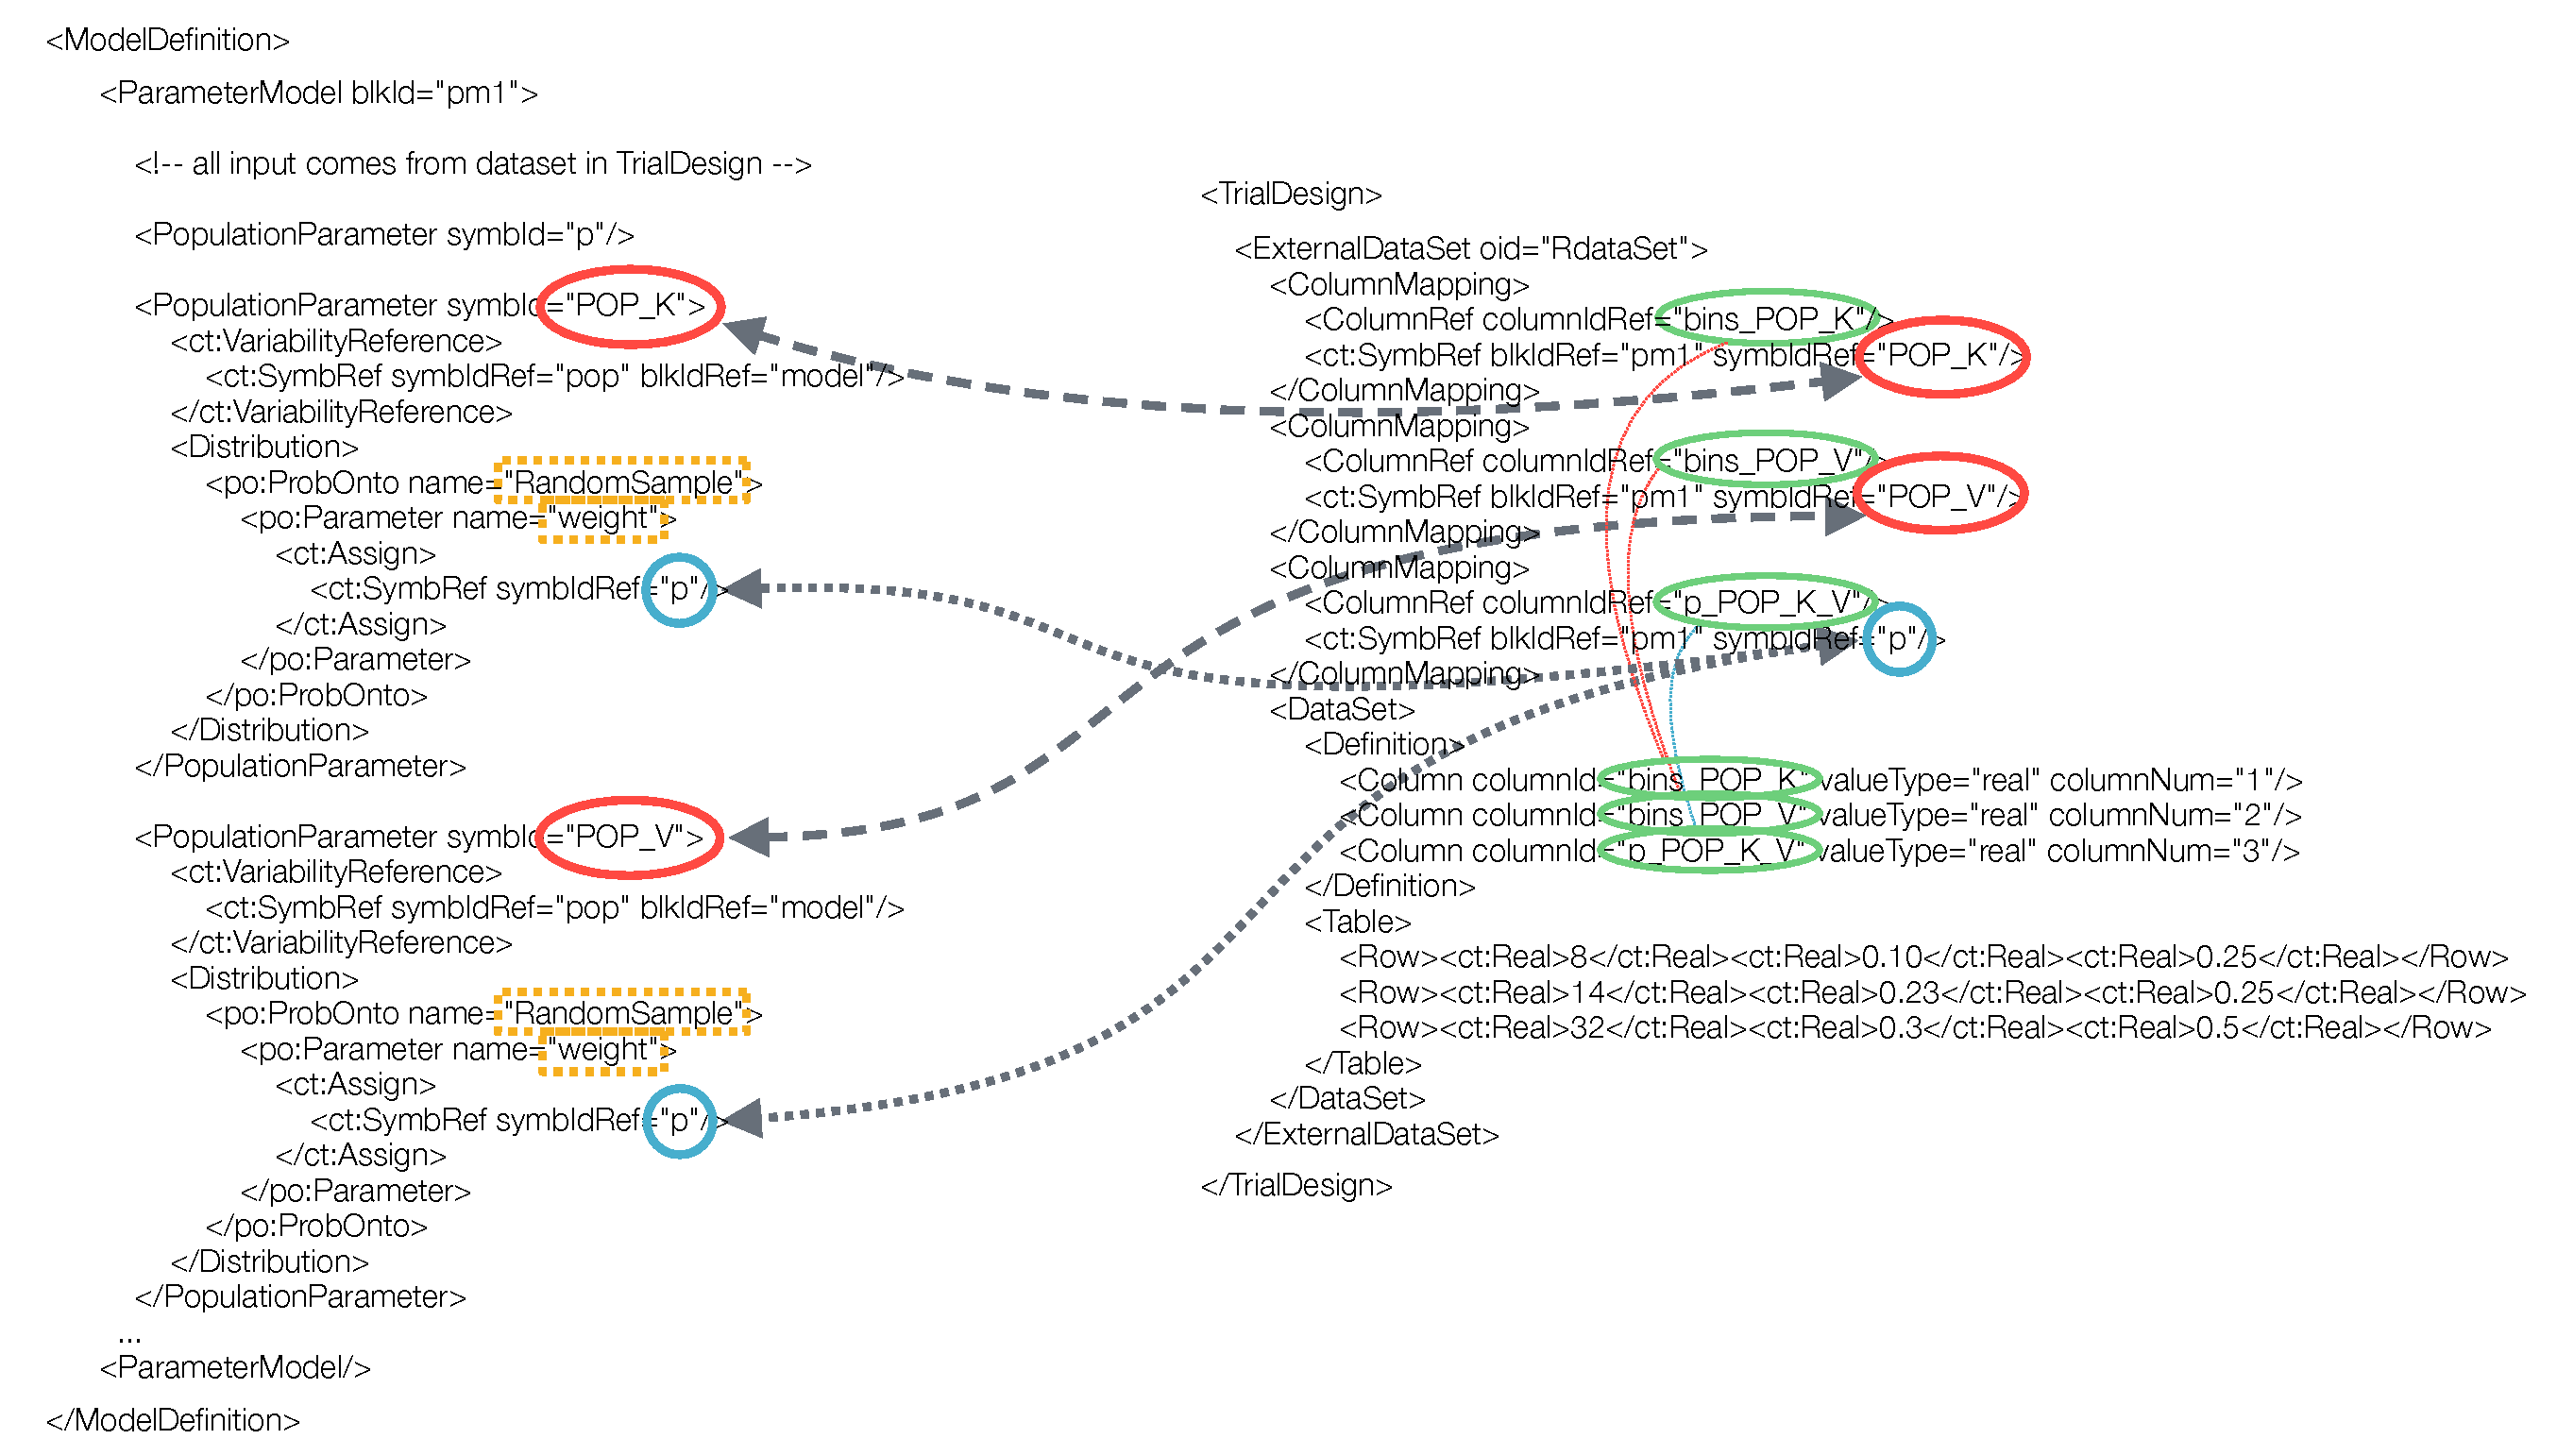
\includegraphics[width=180mm]{pics/Mapping_multiParams_withWeights.pdf}
 \caption{Mapping of samples with weights -- explained graphically.}
 \label{fig:Mapping_withWeights}
\end{figure}

PharmML implementation of the parameter model with distributions defined using
\emph{RandomSample} with \emph{weight} is as following

\lstset{language=XML}
\begin{lstlisting}
    <ParameterModel blkId="pm3">
        <PopulationParameter symbId="p"/>
        <PopulationParameter symbId="POP_K">
            <ct:VariabilityReference>
                <ct:SymbRef symbIdRef="pop" blkIdRef="vm1"/>
            </ct:VariabilityReference>
            <Distribution>
                <po:ProbOnto name="RandomSample">
                    <po:Parameter name="weight">
                        <ct:Assign>
                            <ct:SymbRef symbIdRef="p"/>
                        </ct:Assign>
                    </po:Parameter>
                </po:ProbOnto>
            </Distribution>
        </PopulationParameter>
        <PopulationParameter symbId="POP_V_sample">
            <ct:VariabilityReference>
                <ct:SymbRef symbIdRef="pop" blkIdRef="vm1"/>
            </ct:VariabilityReference>
            <Distribution>
                <po:ProbOnto name="RandomSample">
                    <po:Parameter name="weight">
                        <ct:Assign>
                            <ct:SymbRef symbIdRef="p"/>
                        </ct:Assign>
                    </po:Parameter>
                </po:ProbOnto>
            </Distribution>
        </PopulationParameter>
    </ParameterModel>
\end{lstlisting}
Then the dataset is defined in the \xelem{TrialDesign} as shown below
with the proper column mapping. 
\lstset{language=XML}
\begin{lstlisting}
    <TrialDesign>
        <ExternalDataSet oid="RdataSet">
            <ColumnMapping>
                <ds:ColumnRef columnIdRef="bins_POP_K"/>
                <ct:SymbRef blkIdRef="pm1" symbIdRef="POP_K"/>
            </ColumnMapping>
            <ColumnMapping>
                <ds:ColumnRef columnIdRef="bins_POP_V"/>
                <ct:SymbRef blkIdRef="pm1" symbIdRef="POP_V"/>
            </ColumnMapping>
            <ColumnMapping>
                <ds:ColumnRef columnIdRef="p_POP_V_K"/>
                <ct:SymbRef blkIdRef="pm1" symbIdRef="p"/>
            </ColumnMapping>
            <ds:DataSet>
                <ds:Definition>
                    <ds:Column columnId="bins_POP_K" valueType="real" columnNum="1"/>
                    <ds:Column columnId="bins_POP_V" valueType="real" columnNum="2"/>
                    <ds:Column columnId="p_POP_V_K" valueType="real" columnNum="3"/>
                </ds:Definition>
                <ds:Table>
                    <ds:Row><ct:Real>8</ct:Real><ct:Real>0.10</ct:Real><ct:Real>0.25</ct:Real></ds:Row>
                    <ds:Row><ct:Real>14</ct:Real><ct:Real>0.23</ct:Real><ct:Real>0.25</ct:Real></ds:Row>
                    <ds:Row><ct:Real>32</ct:Real><ct:Real>0.3</ct:Real><ct:Real>0.5</ct:Real></ds:Row>
                </ds:Table>
                <!--  <ds:ExternalFile oid="sxtData">
                        <ds:path>POP_V_K_sample.csv</ds:path>
                      </ds:ExternalFile>-->
            </ds:DataSet>
        </ExternalDataSet>
    </TrialDesign>
\end{lstlisting}



%%%%%%%%%%%%%%%%%%%%%%%%%%%%%%%%%%%%%%%%%%%%%%%%%%%%%%%
\subsection{Mapping using vectors}
\label{subsec:exp3}

In the case the modeller wants to encode a parameter in vector form, here $POP\_K$ 
and $POP\_V$ as  $POP\_K\_V$ vector using samples. Once $POP\_K\_V$ is declared, 
the single parameters are defined using assignments such as $POP\_K = POP\_K\_V[1]$ 
and $POP\_V = POP\_K\_V[2]$. The following series of code snippets shows how this 
is done. First the declaration of $p\_POP\_K\_V$ and $POP\_K\_V$ is made
\lstset{language=XML}
\begin{lstlisting}
            <PopulationParameter symbId="p_POP_K_V"/>
            
            <PopulationParameter symbId="POP_K_V">
                <ct:VariabilityReference>
                    <ct:SymbRef symbIdRef="pop" blkIdRef="model"/>
                </ct:VariabilityReference>
                <Distribution>
                    <po:ProbOnto name="RandomSample">
                        <po:Parameter name="weight">
                            <ct:Assign>
                                <ct:SymbRef symbIdRef="p_POP_K_V"/>
                            </ct:Assign>
                        </po:Parameter>
                    </po:ProbOnto>
                </Distribution>
            </PopulationParameter>
\end{lstlisting}
and then $POP\_K = POP\_K\_V[1]$ assignment is encoded
\lstset{language=XML}
\begin{lstlisting}
            <PopulationParameter symbId="POP_K">
                <ct:Assign>
                    <Uniop xmlns="http://www.pharmml.org/pharmml/0.7/Maths" op="exp">
                        <ct:VectorSelector>
                            <ct:SymbRef symbIdRef="POP_K_V"/>
                            <ct:Cell>
                                <ct:Int>1</ct:Int>
                            </ct:Cell>
                        </ct:VectorSelector>
                    </Uniop>
                </ct:Assign>
            </PopulationParameter>
\end{lstlisting}
and analog for $POP\_V = POP\_K\_V[2]$ (not shown here).

\bigskip
$POP\_K\_V$ is stored in dataset as $bins\_POP\_K$ in \xelem{TrialDesign} section and mapping between 
columns and model elements is performed using \xelem{ColumnMapping}
\lstset{language=XML}
\begin{lstlisting}
<ExternalDataSet oid="RdataSet">
    <ColumnMapping>
        <ColumnRef xmlns="http://www.pharmml.org/pharmml/0.7/Dataset" columnIdRef="bins_POP_K"/>
        <ct:Assign>
            <ct:VectorSelector>
                <ct:SymbRef symbIdRef="POP_K_V" blkIdRef="pm1"/>
                <ct:Cell>
                    <ct:Int>1</ct:Int>
                </ct:Cell>
            </ct:VectorSelector>
        </ct:Assign>
    </ColumnMapping>
    <ColumnMapping>
        <ColumnRef xmlns="http://www.pharmml.org/pharmml/0.7/Dataset" columnIdRef="bins_POP_V"/>
        <ct:Assign>
            <ct:VectorSelector>
                <ct:SymbRef symbIdRef="POP_K_V" blkIdRef="pm1"/>
                <ct:Cell>
                    <ct:Int>2</ct:Int>
                </ct:Cell>
            </ct:VectorSelector>
        </ct:Assign>
    </ColumnMapping>
    <ColumnMapping>
        <ColumnRef xmlns="http://www.pharmml.org/pharmml/0.7/Dataset" columnIdRef="p_POP_K_V"/>
        <ct:SymbRef symbIdRef="p_POP_K_V" blkIdRef="pm1"/>
    </ColumnMapping>
    <DataSet xmlns="http://www.pharmml.org/pharmml/0.7/Dataset">
        <Definition>
            <Column columnId="bins_POP_K" valueType="real" columnNum="1"/>
            <Column columnId="bins_POP_V" valueType="real" columnNum="2"/>
            <Column columnId="p_POP_K_V" valueType="real" columnNum="3"/>
        </Definition>
        <Table>
            <Row><ct:Real>2.006510</ct:Real><ct:Real>5.050013</ct:Real><ct:Real>0.033</ct:Real></Row>
            <Row><ct:Real>2.045465</ct:Real><ct:Real>5.050013</ct:Real><ct:Real>0.100</ct:Real></Row>
            <Row><ct:Real>2.084421</ct:Real><ct:Real>5.050013</ct:Real><ct:Real>0.100</ct:Real></Row>
            <Row><ct:Real>2.123377</ct:Real><ct:Real>5.050013</ct:Real><ct:Real>0.200</ct:Real></Row>
            <!-- rows skipped -->
        </Table>
    </DataSet>
</ExternalDataSet>

\end{lstlisting}
\begin{figure}[ht!]
\centering
  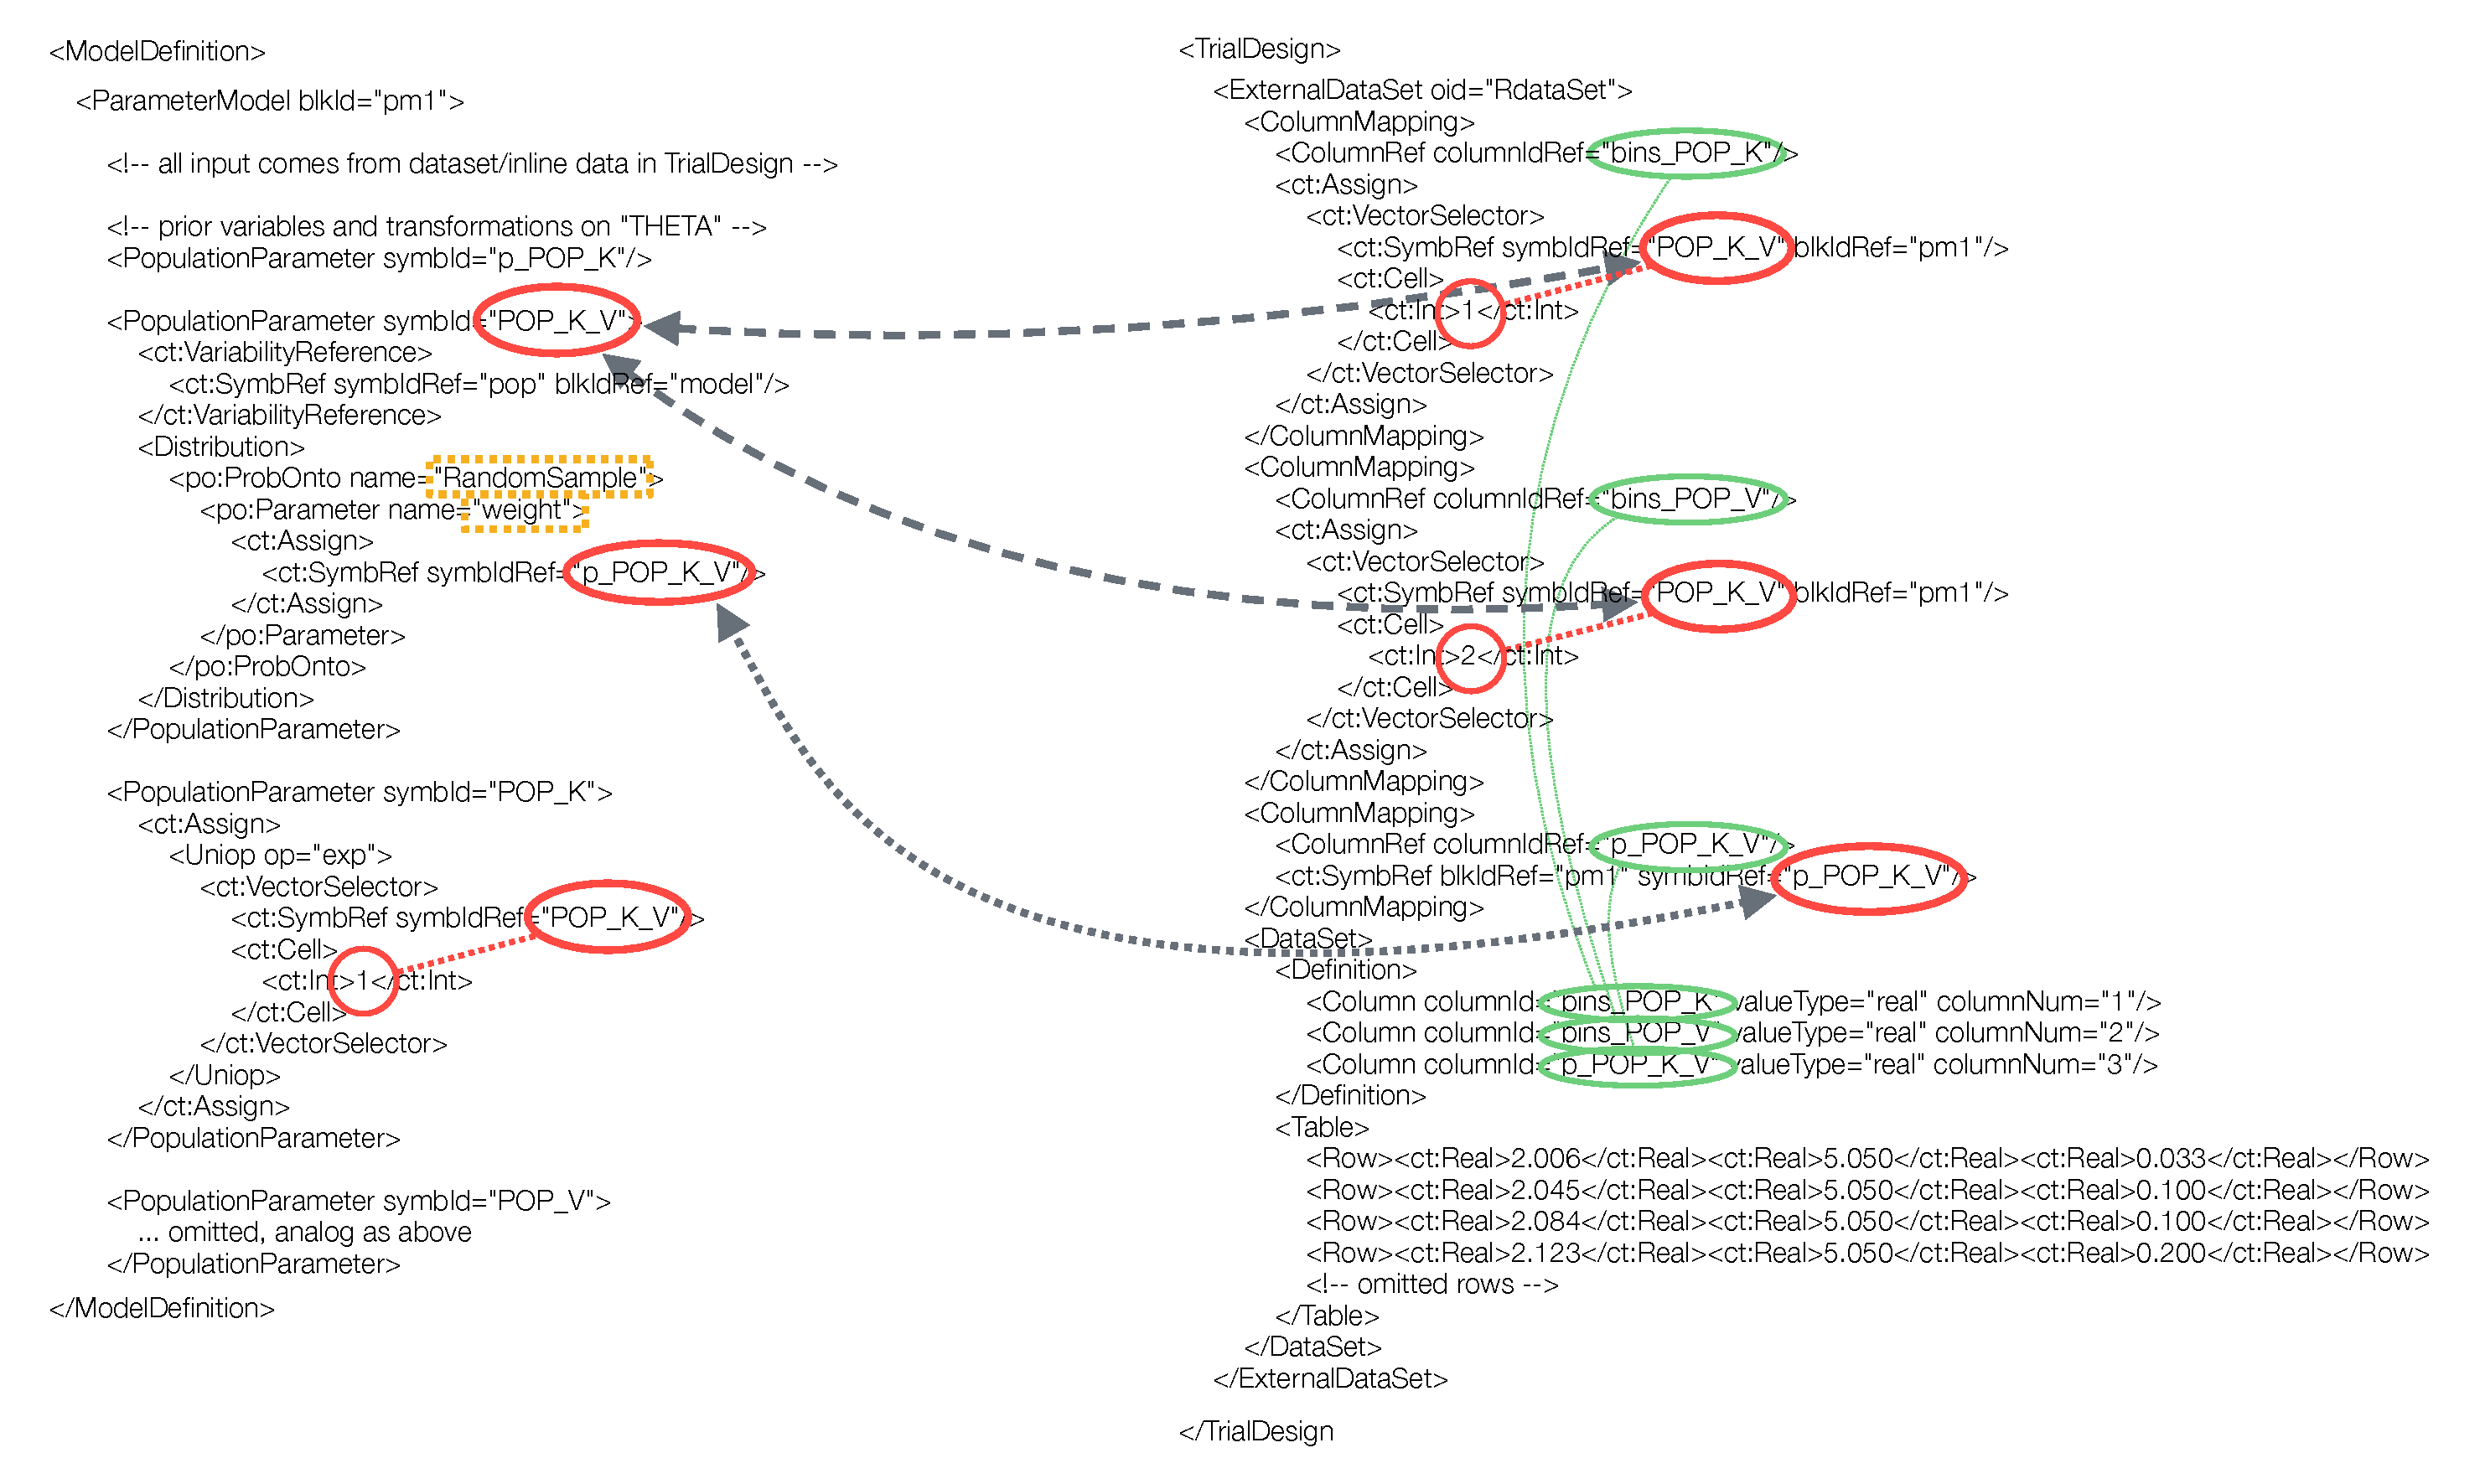
\includegraphics[width=180mm]{pics/Mapping_multiParamsVectorised_withWeights.pdf}
 \caption{Mapping of samples with vectors and weights -- explained graphically.}
 \label{fig:Mapping_multiParamsVectorised_withWeights}
\end{figure}

What is new in this version is the ability to map a particular vector element. Here the essential 
part is repeated to underline how the map of column \emph{bins\_POP\_V} and vector element
$POP\_K\_V[2]$ works.
\lstset{language=XML}
\begin{lstlisting}
    <ColumnMapping>
        <ColumnRef xmlns="http://www.pharmml.org/pharmml/0.7/Dataset" columnIdRef="bins_POP_V"/>
        <ct:Assign>
            <ct:VectorSelector>
                <ct:SymbRef symbIdRef="POP_K_V" blkIdRef="pm1"/>
                <ct:Cell>
                    <ct:Int>2</ct:Int>
                </ct:Cell>
            </ct:VectorSelector>
        </ct:Assign>
    </ColumnMapping>
\end{lstlisting}
See also Figure \ref{fig:Mapping_multiParamsVectorised_withWeights} which shows the mappings graphically.



%%%%%%%%%%%%%%%%%%%%%%%%%%%%%%%%%%%%%%%%%%%%%%%%%%%%%%%
\subsection{Samples in SO}
The concept of encoding samples of empirical distributions, either as inline tables of 
external dataset, is very useful also in the SO context, \cite{SO:2015}. 
For example the posterior distribution of individual parameters estimates is captured 
using an empirical distribution, \emph{RandomSample}.
Here the values for three estimated parameters are encoded inline.
\lstset{language=XML}
\begin{lstlisting}
    <PosteriorDistribution>
        <Distribution>
            <po:ProbOnto name="RandomSample">
                <ds:DataSet>
                    <ds:Definition>
                        <ds:Column columnId="K" columnType="structParameter" valueType="real" columnNum="1"/>
                        <ds:Column columnId="V" columnType="structParameter" valueType="real" columnNum="2"/>
                        <ds:Column columnId="CL" columnType="structParameter" valueType="real" columnNum="3"/>
                    </ds:Definition>
                    <ds:Table>
                        <ds:Row><ct:Real>2.006510</ct:Real><ct:Real>5.050013</ct:Real><ct:Real>0.033333</ct:Real></ds:Row>
                        <ds:Row><ct:Real>2.045465</ct:Real><ct:Real>5.050013</ct:Real><ct:Real>0.100000</ct:Real></ds:Row>
                        <ds:Row><ct:Real>2.084421</ct:Real><ct:Real>5.050013</ct:Real><ct:Real>0.100000</ct:Real></ds:Row>
                        <ds:Row><ct:Real>2.123377</ct:Real><ct:Real>5.050013</ct:Real><ct:Real>0.200000</ct:Real></ds:Row>
                        <ds:Row><ct:Real>2.162333</ct:Real><ct:Real>5.064166</ct:Real><ct:Real>0.100000</ct:Real></ds:Row>
                        <ds:Row><ct:Real>2.201288</ct:Real><ct:Real>5.064166</ct:Real><ct:Real>0.066667</ct:Real></ds:Row>
                        <!-- other sample rows skipped -->
                    </ds:Table>
                    <!-- 
                        <ds:ExternalFile oid="extDataId">
                            <ds:path>samples_KVCL.csv</ds:path>
                        </ds:ExternalFile>-->
                </ds:DataSet>
            </po:ProbOnto>
        </Distribution>
    </PosteriorDistribution>
 \end{lstlisting}
The alternative using external datasets is commented out.

%%%%%%%%%%%%%%%%%%%%%%%%%%%%%%%%%%%%%%%%%%%%%%%%%%%%%%%
\section{Random realisations}
\label{sec:randRealisations}
Another new feature in version 0.8 is the possibility to specify a realisation from any
univariate distribution and is based on analogue featured in UncertML, 
\cite{uncertml3:2014}. The definition reads:
\begin{description}
\item[Realisation] is a single instance of a random variable and can be used 
to imply an observed value, or, as more widely used, a single draw, $x_i$, from a 
probability distribution, $p(x)$.
\end{description}

A new element \xelem{Realisation} has been introduced which child elements
is the familiar \xelem{ProbOnto} within which the name and parameters
of the distribution of interest is specified as the following example shows.

\subsection{Example}
\cite{MLXTRANforSimulator:2014}
Categorical covariates can be defined as a discrete transformation
of continuous random variables. Consider for instance the following 
model encoded in MLXTRAN.
 
\lstset{language=MLX}
\begin{lstlisting}
	[COVARIATE]
	DEFINITION:
	z = {distribution=normal, mean=0, sd=1}
	
	EQUATION:
	if z<-0.2533 ; P(z<-0.2533)=0.4
		cz = 0
	else
		cz = 1
	end
	c=cz
\end{lstlisting}
Note, that \xatt{z=\{distribution=normal,...\}} in the \xatt{DEFINITION} block is a sampling
assignment for which the element \xelem{Realisation} is used.
\lstset{language=MLX}
\begin{lstlisting}
        <CovariateModel blkId="cm2">
            <Covariate symbId="z">
                <Continuous>
                    <Realisation>
                        <po:ProbOnto name="StandardNormal1"/>
                    </Realisation>
                </Continuous>
            </Covariate>
\end{lstlisting}
The remaining definition and assignment of a new covariate is conditional 
on the sampled value \emph{z}
\lstset{language=MLX}
\begin{lstlisting}
            <Covariate symbId="cz">
                <Categorical>
                    <ct:Assign>
                        <ct:Piecewise>
                            <math:Piece>
                                <ct:Real>0</ct:Real>
                                <math:Condition>
                                    <math:LogicBinop op="lt">
                                        <ct:SymbRef symbIdRef="z"/>
                                        <ct:Real>-0.2533</ct:Real>
                                    </math:LogicBinop>
                                </math:Condition>
                            </math:Piece>
                            <math:Piece>
                                <ct:Real>1</ct:Real>
                                <math:Condition>
                                    <math:Otherwise/>
                                </math:Condition>
                            </math:Piece>
                        </ct:Piecewise>
                    </ct:Assign>
                </Categorical>
            </Covariate>
        </CovariateModel>
\end{lstlisting}


%%%%%%%%%%%%%%%%%%%%%%%%%%%%%%%%%%%%%%%%%%%%%%%%%%%%%%%
\section{Markov models}
\label{sec:MM}
New element -- transition aka stochastic matrix -- has been introduced to simplify encoding of Markov models. 
\subsection{Transition matrix}
\label{sec:transitionMatrix}
Stochastic (aka transition matrix) is a matrix used to describe the transitions of a Markov chain.
A stochastic matrix can be 
\begin{itemize}
\item
Left stochastic (default), \xatt{type="leftStochastic"}, a real square matrix, with each row summing to 1.
\item
Right stochastic, \xatt{type="rightStochastic"},  a real square matrix, with each column summing to 1.
\item
Doubly stochastic, \xatt{type="doubleStochastic"},  both columns and rows are summing to 1.
\end{itemize}
Figure \ref{fig:transitionMatrix} visualises a basic example of a Markov model
and the XML code shows how it is implemented 
\begin{figure}[ht!]
\centering
  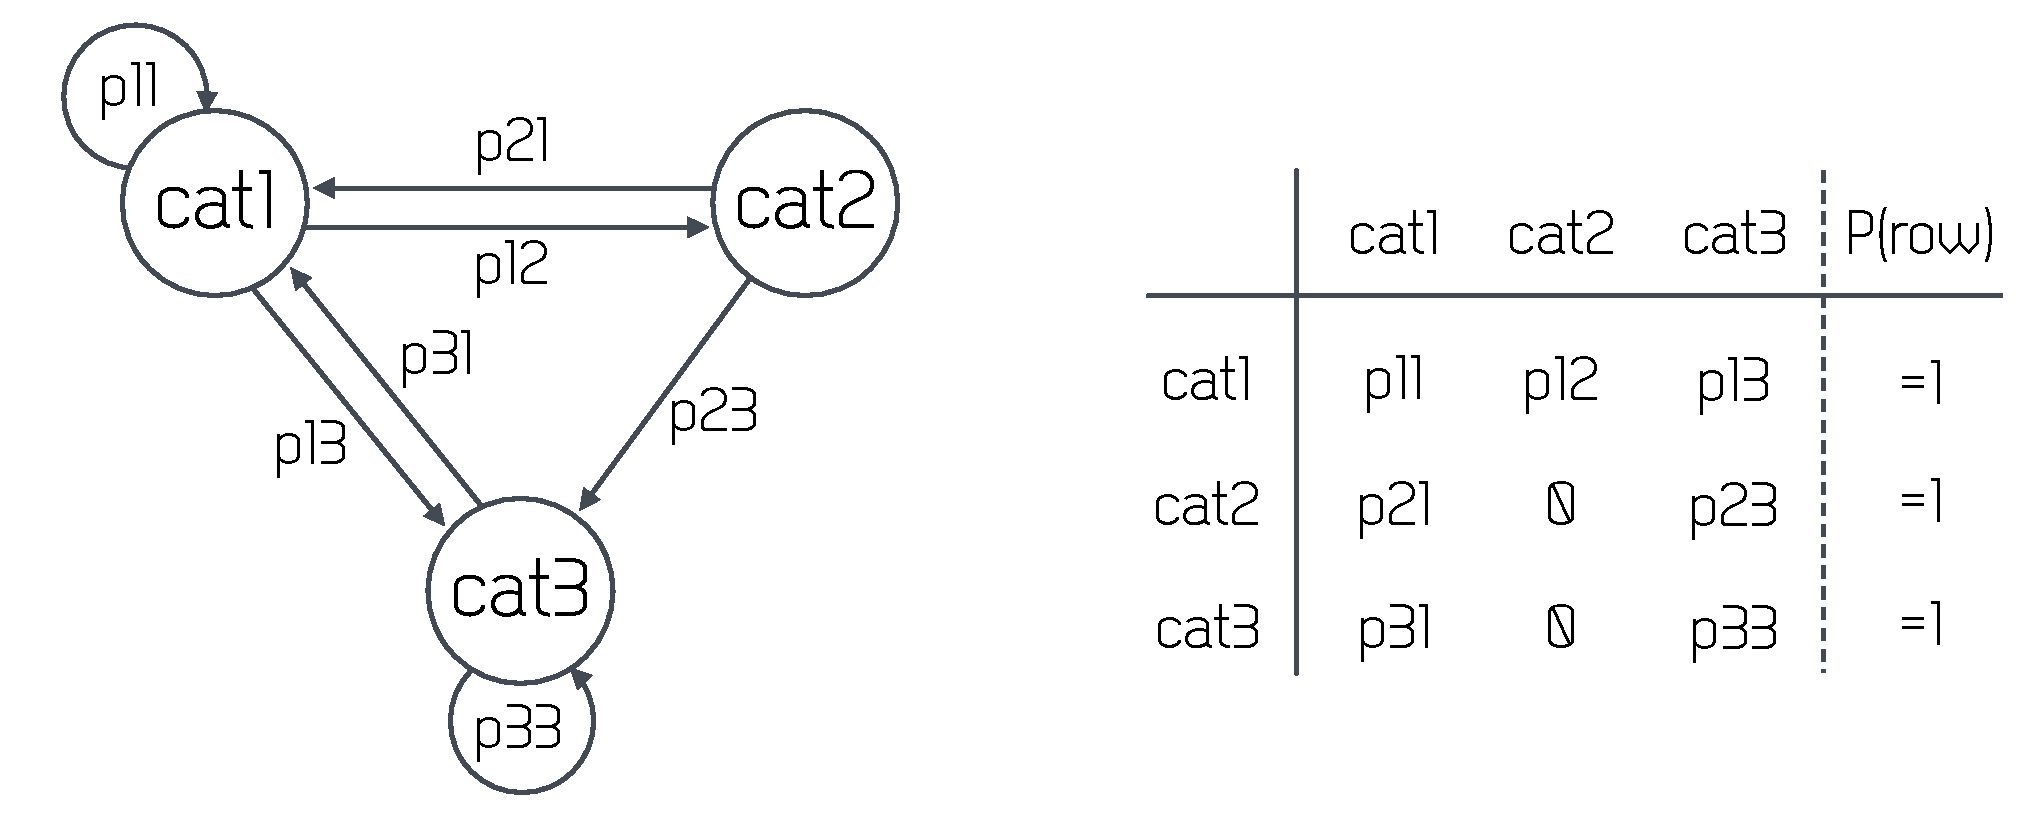
\includegraphics[width=120mm]{pics/transitionMatrix.pdf}
 \caption{An example for a transition matrix for a Markov chain. 
 (Left) the state transition diagram with three possible 
 states cat1, cat2, and cat3. (Right) the \textbf{left} transition matrix.}
 \label{fig:transitionMatrix}
\end{figure}
\lstset{language=XML}
\begin{lstlisting}
        <Dependance type="discreteMarkov"/>
        <TransitionMatrix type="leftStochastic">
            <ct:Matrix matrixType="Any">
                <ct:ColumnNames>
                    <ct:SymbRef symbIdRef="cat1"/>
                    <ct:SymbRef symbIdRef="cat2"/>
                    <ct:SymbRef symbIdRef="cat3"/>
                </ct:ColumnNames>
                <ct:MatrixRow>
                    <ct:SymbRef symbIdRef="p11"/><ct:SymbRef symbIdRef="p12"/><ct:SymbRef symbIdRef="p13"/>
                </ct:MatrixRow>
                <ct:MatrixRow>
                    <ct:SymbRef symbIdRef="p21"/><ct:Real>0</ct:Real><ct:SymbRef symbIdRef="p23"/>
                </ct:MatrixRow>
                <ct:MatrixRow>
                    <ct:SymbRef symbIdRef="p31"/><ct:Real>0</ct:Real><ct:SymbRef symbIdRef="p33"/>
                </ct:MatrixRow>
            </ct:Matrix>
        </TransitionMatrix>
\end{lstlisting}
If the \xatt{type} attribute is not used, the default is the \xatt{leftStochastic} matrix.

\subsection{Conditional transition probabilities/matrix}
\label{sec:condTransitionMatrix}
Conditional transition probabilities can be implemented pairwise, e.g.
\begin{align}
& P(\mbox{Healthy} \rightarrow \mbox{Sick} | \; SEX==F) = 0.1 \nonumber \\
& P(\mbox{Healthy} \rightarrow \mbox{Sick} | \; SEX==M) = 0.2 \nonumber \\
& \mbox{other probabilities omitted...} \nonumber
\end{align}
or using a conditional transition matrix.
\begin{figure}[ht!]
\centering
  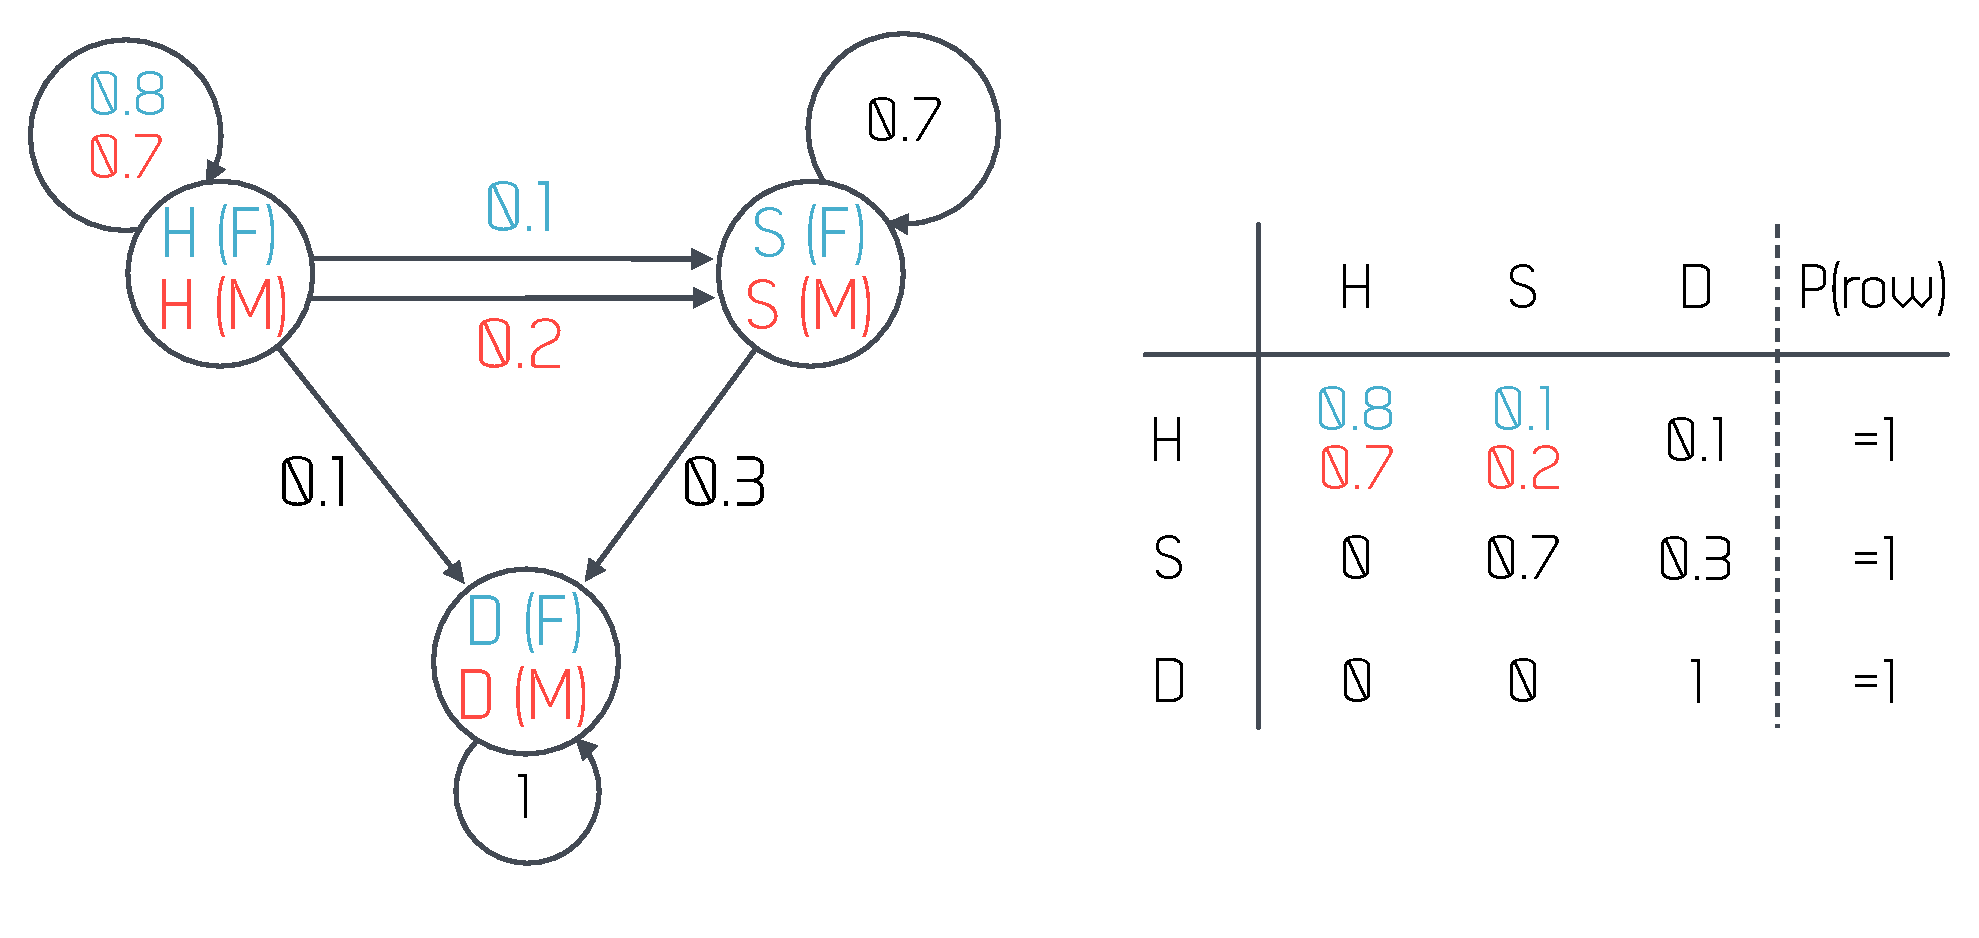
\includegraphics[width=120mm]{pics/markovMatrixCond.pdf}
 \caption{An example of a conditional transition matrix. The left stochastic 
 matrix is assumed by default, i.e. sum of the probabilities in a row must
 be equal 1.}
 \label{fig:markovMatrixCond}
\end{figure}
See section \ref{sec:markovModels} for use examples.


%%%%%%%%%%%%%%%%%%%%%%%%%%%%%%%%%%%%%%%%%%%%%%%%%%%%%%%
\section{N-ary operators}
\label{sec:NaryOps}
N-ary operators are an extension of binary operators in cases when
more then two arguments are provided. The current version supports the 
following operators
%\begin{itemize}
%\item 
%\xatt{plus} - addition operator for n arguments 
%\item 
%\xatt{times} - multiplication operator for n arguments 
%\item 
%\xatt{min} -- minimum of n arguments
%\item 
%\xatt{max} -- maximum of n arguments
%\item 
%\xatt{gcd} -- greatest common divisor of its arguments
%\item 
%\xatt{lcm} -- least common multiple of its arguments
%\end{itemize}

\begin{longtable}{llcc}
\hline
\hline
N-ary operator 				& Name 			& Argument 1 ... N 	& Return type\\
\hline
Addition					& \xatt{plus}		& \xatt{X}, ..., \xatt{X}	& \xatt{Real} \\
Multiplication				& \xatt{times}		& \xatt{X}, ..., \xatt{X}	& \xatt{Real} \\
Smallest of the arguments	& \xatt{min}		& \xatt{X}, ..., \xatt{X}	& \xatt{Real} \\
Largest of the arguments		& \xatt{max}		& \xatt{X}, ..., \xatt{X}	& \xatt{Real} \\
Greatest common divisor		& \xatt{gcd}		& \xatt{X}, ..., \xatt{X}	& \xatt{Real} \\
Least common multiple		& \xatt{lcm}		& \xatt{X}, ..., \xatt{X}	& \xatt{Real} \\
\hline
\caption{N-ary operators supported in v0.8. }
\label{tab:naryops}
\end{longtable}%


\subsection{Rules for using \xelem{Naryop}}
\marginpar{FINISH \\FINISH \\FINISH}
\begin{itemize}
\item
arguments \xatt{X} and \xatt{Y} can be either variable references or real vectors
%\item
%arguments \xatt{level} and \xatt{order} have to be of integer or real type
%\item 
%only two arguments are allowed as children of \xelem{Statsop}, see Table \ref{tab:statistics}
\item 
for statistics where more then two arguments are expected, \xelem{Vector}
with \xelem{VectorElements} has to be used
\end{itemize}


\subsection{Examples}

An example of the use of N-ary operators is shown below using the
\xatt{max} operator to find the maximum value in a sequence of numbers
and to assign it to new parameter, e.g. Amax = max(a1, a2, a3, ...).
\lstset{language=XML}
\begin{lstlisting}
            <IndividualParameter symbId="Amax1">
                <ct:Assign>
                    <math:Naryop op="max">
                        <ct:Vector>
                            <ct:VectorElements>
                                <ct:Real>1</ct:Real>
                                <ct:Real>2</ct:Real>
                                <ct:Real>3</ct:Real>
                                <!-- ... -->
                            </ct:VectorElements>
                        </ct:Vector>
                    </math:Naryop>
                </ct:Assign>
            </IndividualParameter>
\end{lstlisting}
By default \xelem{Vector} structure is used but multiple arguments without are 
also possible as the following code snippet shows
\lstset{language=XML}
\begin{lstlisting}
            <IndividualParameter symbId="Amax1">
                <ct:Assign>
                    <math:Naryop op="max">
                        <ct:Real>1</ct:Real>
                        <ct:Real>2</ct:Real>
                        <ct:Real>3</ct:Real>
                        <!-- ... -->
                    </math:Naryop>
                </ct:Assign>
            </IndividualParameter>
\end{lstlisting}


%%%%%%%%%%%%%%%%%%%%%%%%%%%%%%%%%%%%%%%%%%%%%%%%%%%%%%%
\section{Statistical operators}\marginpar{FINISH}
\label{sec:statsOps}
Based on the UncertML collection, a set of basic statistics is supported in v0.8 
as shown in Table \ref{tab:statistics}. Arguments X and Y can be references 
to variables or explicit vectors of values, see examples below. In few cases 
a second argument is required, \emph{level} or \emph{order}. The order of the 
arguments, 'Argument 2' must follow 'Argument 1', is important as it determines 
the meaning of the argument.
\begin{longtable}{llccc}
\hline
\hline
Statistic 				& Name 					& Argument 1 		& Argument 2 	& Return type\\
\hline
Centred moment		& \xatt{centredMoment}		& \xatt{X}			& \xatt{order}	& \xatt{Real} \\
Coefficient of variation	& \xatt{coefficientOfVariation}	& \xatt{X} 			& -- 			& \xatt{Real} \\
Correlation			& \xatt{correlation}			& \xatt{X} 			& \xatt{Y} 		& \xatt{Real} \\
Decile				& \xatt{decile}				& \xatt{X} 			& \xatt{order} 	& \xatt{Real} \\
Geometric mean		& \xatt{geometricMean}		& \xatt{X} 			& -- 			& \xatt{Real} \\
Kurtosis				& \xatt{kurtosis}			& \xatt{X} 			& -- 			& \xatt{Real} \\
Mean				& \xatt{mean}				& \xatt{X} 			& -- 			& \xatt{Real} \\
Median				& \xatt{median}				& \xatt{X} 			& -- 			& \xatt{Real} \\
Mode				& \xatt{mode}				& \xatt{X} 			& -- 			& \xatt{Real} \\
Moment				& \xatt{moment}			& \xatt{X} 			& \xatt{order} 	& \xatt{Real} \\
Percentile				& \xatt{percentile}			& \xatt{X} 			& \xatt{level} 	& \xatt{Real} \\
Quantile				& \xatt{quantile}			& \xatt{X} 			& \xatt{level} 	& \xatt{Real} \\
Quartile				& \xatt{quartile}				& \xatt{X} 			& \xatt{level} 	& \xatt{Real} \\
Range				& \xatt{range}				& \xatt{X} 			& -- 			& \xatt{Real} \\
Skewness				& \xatt{skewness}			& \xatt{X} 			& -- 			& \xatt{Real} \\
Standard deviation		& \xatt{standardDeviation}	& \xatt{X} 			& -- 			& \xatt{Real} \\
Variance				& \xatt{variance}			& \xatt{X} 			& -- 			& \xatt{Real} \\
\hline
\caption{Statistics supported in v0.8. The type of the arguments \xatt{X} and \xatt{Y} 
can be either variable references or real vectors. Multiple values 
without \xelem{Vector} element is not allowed. In few cases a second argument 
is required, \xatt{level} or \xatt{order}, both of real type. The correct sequence of the arguments, 
first 'Argument 1' then 'Argument 2', is important as it determines the meaning 
of the arguments.}
\label{tab:statistics}
\end{longtable}%

\subsection{Rules for using \xelem{Statsop}}
\marginpar{FINISH \\FINISH \\FINISH}
\begin{itemize}
\item
arguments \xatt{X} and \xatt{Y} can be either variable references or real vectors
\item
arguments \xatt{level} and \xatt{order} have to be of integer or real type
\item 
only two arguments are allowed as children of \xelem{Statsop}, see Table \ref{tab:statistics}
\item 
for statistics where more then two arguments are expected, \xelem{Vector}
with \xelem{VectorElements} has to be used
\end{itemize}


\subsection{Examples}
Some examples of the use of statistical operators are shown below. 
\subsubsection*{Example -- more then two arguments }
\lstset{language=XML}
\begin{lstlisting}
    <ct:Variable symbId="Qm" symbolType="real">
        <ct:Assign>
            <math:Statsop op="mean">
                <ct:Vector>
                    <ct:VectorElements>
                        <ct:SymbRef blkIdRef="pm1" symbIdRef="Q0"/>
                        <ct:SymbRef blkIdRef="pm1" symbIdRef="Q1"/>
                        <ct:SymbRef blkIdRef="pm1" symbIdRef="Q2"/>
                    </ct:VectorElements>
                </ct:Vector>
            </math:Statsop>	
        </ct:Assign>
    </ct:Variable>
\end{lstlisting}



\section{Covariates versus regressors}
\label{sec:covVsRegs}
There are different types of covariates and we distinguish between
following types
\begin{itemize}
\item 
constant covariates
\item 
occasion dependent covariates
\item 
time dependent covariates -- \emph{aka} regressors 
\end{itemize}
Due to the various interpretation and naming conventions for covariates
and regressors there is a need to identify those and this can be done 
also in the \xelem{CovariateModel} by assigning an optional attribute
\xatt{type} with values \emph{occasionDependent}, \emph{timeDependent}, 
\emph{constant}. The following snippet shows how this is done for 
a time dependent covariate 

\lstset{language=XML}
\begin{lstlisting}
        <CovariateModel blkId="cm1">
            <Covariate type="timeDependent" symbId="CovariateX">
                <!-- ... -->
            </Covariate>
        </CovariateModel>
\end{lstlisting}
For more on regressors support in PharmML, see Section "6.4 Regressor support"
in v0.7 spec \cite{Swat:2015b}.


%%%%%%%%%%%%%%%%%%%%%%%%%%%%%%%%%%%%%%%%%%%%%%%%%%%%%%%
\section{Extension in categorical covariates model}
\label{sec:catCovModel}

\subsection{Covariate declaration/assignment}
Declaration and assignment of new categorical covariates is now possible.  
Here a simple example of a conditional definition from one of the IOG use cases
\lstset{language=NM}
\begin{lstlisting}
            DDU = if (DDUR > 2) then 1 # duration > 1 month
            else 0 # duration of current episode < 1 month
\end{lstlisting}
which implementation in XML using the piecewise structure reads
\lstset{language=XML}
\begin{lstlisting}
    <Covariate symbId="DDU">
        <Categorical>
            <ct:Assign>
                <ct:Piecewise>
                    <math:Piece>
                        <ct:Real>1</ct:Real>
                        <math:Condition>
                            <math:LogicBinop op="lt">
                                <ct:SymbRef symbIdRef="DDUR"/>
                                <ct:Real>2</ct:Real>
                            </math:LogicBinop>
                        </math:Condition>
                    </math:Piece>
                    <math:Piece>
                        <ct:Real>0</ct:Real>
                        <math:Condition>
                            <math:Otherwise/>
                        </math:Condition>
                    </math:Piece>
                </ct:Piecewise>
            </ct:Assign>
        </Categorical>
    </Covariate>
\end{lstlisting}


\subsection{Distribution of categorical covariates}

The possibility to define distribution of categorical covariates was possible 
before but was inconsistent with the way continuous covariates are handled.
While the previous option (using \xelem{Probability} for each category is still
supported), the \xelem{Distribution} element with child \xelem{ProbOnto} 
can be used now as well.

\begin{longtable}{cc}
\hline
\hline
option supported in $\le$ 0.7.3 & new option in version 0.8 \\
\hline
\lstset{language=XML}
\begin{lstlisting}
<Covariate symbId="Sex">
    <Categorical>
        <Category catId="F">
            <Probability>
                <ct:SymbRef symbIdRef="p1"/>
            </Probability>
        </Category>
        <Category catId="M">
            <Probability>
                <ct:SymbRef symbIdRef="p2"/>
            </Probability>
        </Category>
    </Categorical>
</Covariate>
\end{lstlisting}
&
\lstset{language=XML}
\begin{lstlisting}
<Covariate symbId="Sex">
    <Categorical>
        <Category catId="F"/>
        <Category catId="M"/>
        <Distribution>
            <po:ProbOnto name="CategoricalNonordered1">
                <po:Parameter name="categoryProb">
                    <ct:Assign>
                        <ct:Vector>
                            <ct:VectorElements>
                                <ct:SymbRef symbIdRef="p1"/>
                                <ct:SymbRef symbIdRef="p2"/>
                            </ct:VectorElements>
                        </ct:Vector>
                    </ct:Assign>
                </po:Parameter>
            </po:ProbOnto>
        </Distribution>
    </Categorical>
</Covariate>
\end{lstlisting}
\\
\hline
\caption{Distribution of categorical covariates using \xelem{Distribution} and 
\xelem{ProbOnto} elements.}
\end{longtable}%

\subsection{Conditional distribution of categorical covariates}
Also new is the possibility to define a distribution conditional on other covariates, 
e.g. the previous example is extended in that the SEX distribution varies between
studies, with probabilities given by the two following vectors $\boldsymbol p1 = 
\{p1_{S1},p2_{S1}\}$ or $\boldsymbol p2 = \{p1_{S2},p2_{S2}\}$.
Such model reads then 
\bigskip
\begin{algorithmic}
	\If {$STUDY == S1$}
	    \State SEX $\sim$ Categorical($\boldsymbol p1$)
	\ElsIf{$STUDY == S2$} 
	    \State SEX $\sim$ Categorical($\boldsymbol p2$)
	\EndIf
\end{algorithmic}
\bigskip
First the STUDY  covariate is declared with category identifiers S1 and S2
\lstset{language=XML}
\begin{lstlisting}
            <Covariate symbId="STUDY">
                <Categorical>
                    <Category catId="S1"/>
                    <Category catId="S2"/>
                </Categorical>
            </Covariate>
\end{lstlisting}
then the distribution of SEX can be defined using here the \emph{CategoricalNonordered1} 
distribution defined in ProbOnto 
\lstset{language=XML}
\begin{lstlisting}
            <Covariate symbId="SEX">
                <Categorical>
                    <Category catId="F"/>
                    <Category catId="M"/>
                    <Distribution>
                        <Piecewise>
                            <math:Piece>
                                <po:ProbOnto name="CategoricalNonordered1">
                                    <po:Parameter name="categoryProb">
                                        <ct:Assign>
                                            <ct:Vector>
                                                <ct:VectorElements>
                                                    <ct:SymbRef symbIdRef="p1_S1"/>
                                                    <ct:SymbRef symbIdRef="p2_S1"/>
                                                </ct:VectorElements>
                                            </ct:Vector>
                                        </ct:Assign>
                                    </po:Parameter>
                                </po:ProbOnto>
                                <math:Condition>
                                    <math:LogicBinop op="eq">
                                        <ct:SymbRef symbIdRef="STUDY"/>
                                        <ct:CatRef catIdRef="S1"/>
                                    </math:LogicBinop>
                                </math:Condition>
                            </math:Piece>
                            <math:Piece>
                                <po:ProbOnto name="CategoricalNonordered1">
                                    <po:Parameter name="categoryProb">
                                        <ct:Assign>
                                            <ct:Vector>
                                                <ct:VectorElements>
                                                    <ct:SymbRef symbIdRef="p1_S2"/>
                                                    <ct:SymbRef symbIdRef="p2_S2"/>
                                                </ct:VectorElements>
                                            </ct:Vector>
                                        </ct:Assign>
                                    </po:Parameter>
                                </po:ProbOnto>
                                <math:Condition>
                                    <math:LogicBinop op="eq">
                                        <ct:SymbRef symbIdRef="STUDY"/>
                                        <ct:CatRef catIdRef="S2"/>
                                    </math:LogicBinop>
                                </math:Condition>
                            </math:Piece>
                        </Piecewise>
                    </Distribution>
                </Categorical>
            </Covariate>
        </CovariateModel>
\end{lstlisting}


%%%%%%%%%%%%%%%%%%%%%%%%%%%%%%%%%%%%%%%%%%%%%%%%%%%%%%%
\section{Minor extensions}
\label{sec:minorExt}

\subsection{Datasets declaration}
\label{sec:dataSets}

The declaration of the external dataset provides more flexibility. 
While in previous versions the allowed values for the mandatory \xatt{toolName}
attribute were predefined with only options \{Monolix, NONMEM, BUGS\}, e.g.
\lstset{language=XML}
\begin{lstlisting}
        <ExternalDataSet toolName="BUGS" oid="RdataSet">
            <ColumnMapping>
            <!-- ... -->
\end{lstlisting}
in version 0.8 any name can be used or the attribute can be skipped entirely
so that the following
\lstset{language=XML}
\begin{lstlisting}
        <ExternalDataSet oid="RdataSet">
            <ColumnMapping>
            <!-- ... -->
\end{lstlisting}
is sufficient. This change is essential to allow the use of any datasets and formats.


\subsection{Conditional 'ignorance'}
\label{subsec:condIgnore}

The conditional ignoring of data records is now supported, for example
\lstset{language=NM}
\begin{lstlisting}
	IGNORE=(MDV0.EQ.1)
	IGNORE=(STAGE.GT.5)
	IGNORE=(STAGE.EQ.3)
\end{lstlisting}
would be implemented as
\lstset{language=XML}
\begin{lstlisting}
        <ExternalDataSet oid="NMoid">
            <ds:DataSet>
                <ds:Definition>
                    <ds:Column columnId="ID" columnType="id" valueType="string" columnNum="1"/>
                    <ds:Column columnId="TIME" columnType="time" valueType="real" columnNum="2"/>
                    <ds:Column columnId="Y" columnType="dv" valueType="real" columnNum="3"/>
                    <ds:Column columnId="MDV0" columnType="covariate" valueType="real" columnNum="4"/>
                    <ds:Column columnId="STAGE" columnType="covariate" valueType="real" columnNum="5"/>
                    <ds:IgnoreLine>
                        <math:Condition>
                            <math:LogicBinop op="eq">
                                <ds:ColumnRef columnIdRef="MDV0"/>
                                <ct:Real>1</ct:Real>
                            </math:LogicBinop>
                        </math:Condition>
                    </ds:IgnoreLine>
                    <ds:IgnoreLine>
                        <math:Condition>
                            <math:LogicBinop op="gt">
                                <ds:ColumnRef columnIdRef="STAGE"/>
                                <ct:Real>5</ct:Real>
                            </math:LogicBinop>
                        </math:Condition>
                    </ds:IgnoreLine>
                    <ds:IgnoreLine>
                        <math:Condition>
                            <math:LogicBinop op="eq">
                                <ds:ColumnRef columnIdRef="STAGE"/>
                                <ct:Real>3</ct:Real>
                            </math:LogicBinop>
                        </math:Condition>
                    </ds:IgnoreLine>
                </ds:Definition>
                <ds:ExternalFile oid="dataOid">
                    <ds:path>example4.csv</ds:path>
                    <ds:format>CSV</ds:format>
                    <ds:delimiter>COMMA</ds:delimiter>
                </ds:ExternalFile>
            </ds:DataSet>
        </ExternalDataSet>
\end{lstlisting}
Note, that MDV0 and STAGE have to be defined as covariates (or regressors)
in the according in covariate model. The default option, without conditioning, is unchanged, e.g.
\lstset{language=XML}
\begin{lstlisting}
        <ds:IgnoreLine symbol="@"/>
\end{lstlisting}

